%!TeX root=../../main.tex
\chapter{Evaluation}                                 \label{ch:evaluation}
This chapter aims to evaluate our algorithm described in chapter 3. This evaluation will be based on 4 research questions, split up into 2 experiments. The first experiment will be a comparison between Kano and the comparable part of our algorithm that is responsible for incrementally updating the matrix. The second experiment is a general test of our overall algorithm in terms of time and memory consumption. Both of the evaluation experiments are run on the same cluster setup and share configuration specifics, which we will describe in the first section. The second and third sections will talk about the first and second experiment respectively and include subsections about the experiments' approach, setup and results. We end with an overview of  conclusions drawn from the experiments
\\[10pt]

% =========================================
\section{Evaluation setup} \label{sec:evalsetup}


The \acrshort{k8s} cluster used for the experiments consists of 8 nodes: 7 workers nodes and a single control-plane node that does not run any containers. Each of these nodes are located on its own \acrshort{vm}, which are deployed as instances on the Openstack installation of the Department of Computer Science at KULeuven. Each instance has 2 VCPUs, 4GB RAM and 20GB memory, and runs Ubuntu 22.04 jammy for its OS. There are no Security Groups applied to the instances except for the default. Calico is used as \acrshort{cni} to provide the connection between the \acrshort{k8s} nodes, which all run on the \acrshort{k8s} Git version v1.22.17. \acrshort{k8s} runs on default settings and specifies the maximum amount of pods per worker node at around 100 pods.
\\[10pt]

Each pod we deploy is created with the latest nginx image, which is version 1.25.3 at the time of the experiments and writing. \autoref{fig:podyaml} shows the pod manifest structure for each deployed pod, with $name$ and $labels$ randomly generated and $ns$ depending on the execution arguments which we will describe in the next sections. As shown in the picture the pods are specified to not use any resources when deployed. The experiment algorithms are executed on the control-plane node and will execute without the need for interaction, on the condition that the specified namespace used for the experiment already exists on the cluster.
\\[10pt]
\begin{figure}[htbp]
  \centering
  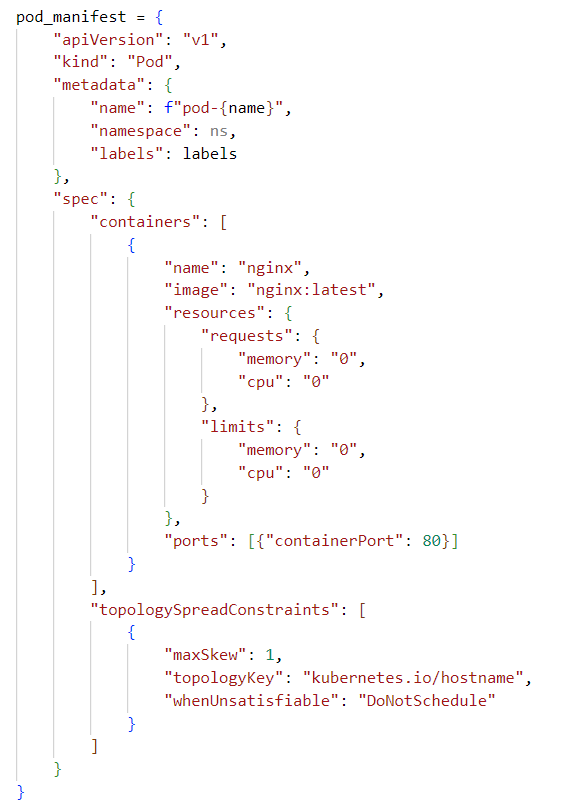
\includegraphics[width=0.6\textwidth]{images/podyaml.png} 
  \caption{Template for pod creation}
  \label{fig:podyaml}
\end{figure}

Each experiment will be run once for each of the events described in \autoref{tab:events} since they can differ in space and time cost. For example, removing a container might be faster than adding a new container, since the first mainly just removes data while the latter includes a search for matching \acrshort{np}s according to its labels. However, we only measure four out of the six events that we can capture, since updating \acrshort{np}s and containers equals directly to first executing a deletion event, directly followed by a creation event. The update events can thus be calculated from the creation and deletion events saving time when executing the experiments.
\\[10pt]

We want to know how each experiment behaves when the cluster size increases in terms of pods and network policies. For this reason, we define 5 cluster setups that define variables such as number of pods and number of network policies. The combinations of 5 cluster setups and 4 events gives us a total of 20 smaller experiments for each experiment,  which we will call sub-experiments.  Each of these 20 sub-experiments is run a hundred times giving us a total of 2000 runs and their respective data per experiment.
\\[10pt]


% =========================================
\section{Experiment 1}\label{sec:experiment1}
Kano is a research solution that verifies \acrshort{np}s based on the reachabilitymatrix it generates when provided with a list of pods and a list of policies. For some background about Kano, we refer to \autoref{sec:kano}. Kano only has a generative algorithm to create this reachabilitymatrix, while our solution provides an incremental approach that updates the reachabilitymatrix instead of regenerating it. Naturally, a comparison between each approach is required and will be described in this section. This comparison will be used to answer the following two research questions:

\begin{itemize}
    \item \textit{Q1:} What is the difference in time cost between an incremental update of the Kano matrix compared to newly generating the Kano matrix for every event and how does this difference scale with pod/policy numbers
    \item \textit{Q2:} What is the difference in space cost between an incremental update of the Kano matrix compared to newly generating the Kano matrix for every event and how does this difference scale with pod/policy numbers
\end{itemize}

Before we delve into the experiment approach, setup and results we declare our expectations for these questions:

\begin{itemize}
    \item \textit{Expectation E1:} We expect that the time cost of our incremental approach will be higher in small clusters due to the writing times of variables, but will prove better than the time cost of the generative approach as the cluster increases since the incremental approach does not have to verify all \acrshort{np}s and containers.
    \item \textit{Expectation E2:} We expect that the space cost of the incremental approach will be higher than that of the generative approach due to the memory required for storing the current cluster state. We predict this difference will only increase as the cluster increases in size.
\end{itemize}

% =========================================
\subsection{Approach} \label{exp1:approach}
Since our algorithm does much more than just updating the reachabilitymatrix we first have to remove the irrelevant parts from our codebase. The \acrlong{sgic} is removed from the algorithm altogether, while the Analyzer gets modified so that it only calls upon the \acrlong{kic} to update the reachabilitymatrix. As a result, the analyzer does not use the updated matrix to compare it with the previous cluster state nor does it print out any information anymore. This adapted algorithm for the incremental approach now allows for a direct comparison with Kano's generative approach.  For both approaches, we want to collect the time (ms), memory at the start of the method (MB), the highest memory peak during execution of the method (MB) and the difference between the peak and start memory (MB). Memory and time usage are collected by leveraging the tracemalloc and time python libraries respectively \cite{tracemalloc} \cite{time}.
\\[10pt]

Each event type will be tested in 5 different setups which will be identical for each event and are described in \autoref{tab:exp1pars}. These parameter values are based on the parameters used in the evaluation of Kano \cite{kano}. However, our maximum number of pods and policies is lower than Kano's evaluation due to the limits of our experiment cluster. We will now summarize the meaning of each parameter:
\begin{itemize}
    \item \textit{Pod num}: This variable describes the number of pods that will be generated and deployed on the cluster. Each pod has a single container thus this variable directly annotates the amount of containers as well.
    \item \textit{Pol num}: This variable describes the number of \acrshort{np}s that will be generated and deployed on the cluster.
    \item \textit{key limit}: This variable describes the number of distinct keys out of which one will randomly be selected each time a key-value label is generated. The lower this number, the higher the chance of matches between containers and \acrshort{np} label selectors.
    \item \textit{Value limit}: This constant describes the number of distinct values out of which one will randomly be selected each time a key-value label is generated.
    \item \textit{Pol select limit}: This constant describes the amount of selector fields in a network policy.
    \item \textit{Pol select label limit}: This constant describes the maximum amount of label selectors in a selector field of a network policy. each selector field will thus have between 1 and this value's amount of randomised label selectors.
    \item \textit{Pol allow limit}: This constant describes the maximum amount of allowed fields in a network policy. each \acrshort{np} will thus have between 1 and this value's amount of allowed fields.
    \item \textit{Pol allow label limit}: This constant describes the maximum amount of allow selectors in an allow field of a network policy. each allow field will thus have between 1 and this value's amount of randomised label selectors.
     \item \textit{Pod label limit}: This constant describes the maximum amount of labels in a container. Each container will thus have between 1 and this value's amount of randomised key-value labels.
\end{itemize}

\begin{table}[H]
    \centering
    \begin{tabular}{|l|c|c|c|c|c|}
        \hline
        \textbf{Name} & \textbf{setup 1} & \textbf{setup 2} & \textbf{setup 3} & \textbf{setup 4} & \textbf{setup 5}\\
        \hline
        Pod num & 50 & 100 & 250 & 500 & 750 \\
        Pol num & 20 & 50 & 100 & 200 & 300 \\
        Key limit & 2 & 5 & 8 & 10 & 20 \\
        Value limit & 10 & 10 & 10 & 10 & 10 \\
        Pol select limit & 1 & 1 & 1 & 1 & 1 \\
        Pol select label limit & 3 & 3 & 3 & 3 & 3 \\
        Pol allow limit & 3 & 3 & 3 & 3 & 3 \\
        Pol allow label limit & 3 & 3 & 3 & 3 & 3 \\
        Pod label limit & 5 & 5 & 5 & 5 & 5 \\
        \hline
    \end{tabular}
    \caption{Experiment 1 parameter values}
    \label{tab:exp1pars}
\end{table}

% =========================================
\subsection{Execution} \label{exp1:execution}
 We will now describe the execution of a single sub-experiment step by step.
\\[10pt]

\textbf{STEP 0:} Call the python file experiment1.py with the following arguments: $number\_of\_runs$, $number\_of\_pods$, $number\_of\_policies$, $namespace$, $key\_limit$ and $event\_type$ according to the sub-experiment settings. The algorithm will then execute STEP 1 to STEP 7 as many times as defined in argument $number\_of\_runs$.
\\[10pt]

\textbf{STEP 1:} We fully reset the namespace defined in the $namespace$ argument with the help of the Python \acrshort{k8s} API. This is coded in a separate delete.py file and extended with some extra tests and timeouts to guarantee that all objects are successfully removed before continuing.
\\[10pt]

\textbf{STEP 2:} We deploy as many pods and \acrshort{np}s as defined in arguments \newline $number\_of\_pods$ and $number\_of\_policies$. For this functionality a separate deploy.py python file has been created that will generate and deploy the \acrshort{np}s and pods, when called upon with the variables $namespace$ and $key\_limit$ as parameters. The other relevant constants in \autoref{tab:exp1pars} are hard coded since they don't change between sub-experiments. The deploy file is equipped with a list of distinct keys and values to leverage when creating the randomised pods and \acrshort{np}s. However, the key list is first shortened until it has a length equal to the $key\_limit$ parameter before being utilised. The randomised pods and \acrshort{np}s get deployed in the namespace defined in the $namespace$ argument with the help of the Python \acrshort{k8s} API. We use extra tests and timeouts to guarantee all objects are successfully deployed and ready before continuing.
\\[10pt]

\textbf{STEP 3:} We start the watcher with the flags for debug mode, verbose mode and start the checkup all set to False. With the use of threading events, we guarantee that the threads that watch the APIs for pods and \acrshort{np}s are successfully running, to prevent the next step from executing too early, therefore missing the event and being unable to handle it.
\\[10pt]

\textbf{STEP 4:} We execute one event, depending on the $event\_type$ argument. If it is a delete event we call the delete.py file again and let it randomly remove one of the existing objects that correspond to the event type. If it is a deploy event we call the deploy.py file to generate one more randomly generated object according to the correct parameters.
\\[10pt]

\textbf{STEP 5:} We once again leverage threading events to get notified when the consumer thread has received and handled its first event. Since the watcher was initialized after all pods and \acrshort{np}s were fully ready it will always be the event from step 4 that will be caught. When the consumer catches the event it will start the timer right before calling the analyzer for event handling. Once the analyzer returns the function call the timer immediately gets stopped to get a final execution time. Similarly, we measure the memory usage at the start of the algorithm, and the highest peak of memory usage during the event handling. With this we can calculate the difference and thus how much memory was used (in bytes). These memory and time measurements get stored in variables in the watcher.
\\[10pt]

\textbf{STEP 6:} Once we get the message that the event is handled we retrieve the measurements from the watcher and store it locally. We can then stop the watcher.
\\[10pt]

\textbf{STEP 7:} We now call retrieve all existing pods and \acrshort{np}s in the cluster and put them in lists.  Once we have started a new timer and started tracing memory we give these lists to the original matrix generation method from Kano. Upon return of the reachabilitymatrix, the timer and memory measurement are stopped and stored in variables. We also include a comparison between the incremental and generative reachabilitymatrices to ensure the results are correct and no bugs or edge cases were discovered. If the latter is the case the sub-experiment is cancelled and debug information is printed out.
\\[10pt]

\textbf{STEP 8:} Once the hundred runs of the sub-experiment have finished we store all the data in a CSV file and store it on the control plane node that ran the experiment. We can then retrieve this file and combine it with other sub-experiment files for evaluation. 
\\[10pt]


% =========================================
\subsection{Experiment results} \label{exp1:results}

The results of the experiment will be divided into eight different graphs: for each event type, we created a graph displaying average and median time as well as a graph that shows average and median memory consumption. This division of data is required since each type of event has a different method for updating the current cluster state in our algorithm and therefore might introduce differences between them. All the graphs use the same values and increments on their axis to allow a direct comparison. We will start by looking at the time graphs after which continue with the memory results.
\\[10pt]

\textbf{Time consumption}
\newline When looking at the graphs in \autoref{fig:exp1-addNP-time}, \autoref{fig:exp1-addPod-time}, \autoref{fig:exp1-delNP-time}  and \autoref{fig:exp1-delPod-time} we can quickly deduce that our incremental approach starts more time expensive but becomes faster as the scale of the cluster increases. This trend seems to continue as the cluster grows and is in line with our expectation for Q1 described in \autoref{sec:experiment1}. We will now take a deeper look into the data and describe some additional observations:

\begin{itemize}
    \item If we look at the intersection point of the generative and incremental averages we see a difference between \acrshort{np} and pod events. For the \acrshort{np} events, the intersection always appears between the third and fourth sub-experiment, while for the pod events, this is closer the the third sub-experiment. This can be explained due to the different approaches: when a \acrshort{np} is added or deleted all the pods with the corresponding labels must be retrieved, while a pod addition or deletion needs to find the corresponding network policies. Since our experiment settings always have more pods than \acrshort{np}s the search time for \acrshort{np} events naturally becomes higher.
    
    \item Thanks to the included median values we see that the deletion events have fewer outlying values compared to the creation events. This can be explained once again by the approach to handle these events: when creating a pod or \acrshort{np} the time will be influenced by the number of matching label selectors between pods and network policies, which is randomised for each run. When deleting an object we do not need to search for a match between selectors, instead, we simply remove the information from the cluster state, thereby saving time.
    
    \item Although the generative approach from Kano stays consequent throughout the four events our solution is more dependent on the type of event being handled. The incremental approach stays in the similar range of values for the first sub-experiments, but as the cluster size increases the pod events generally take less time to update the reachabilitymatrix compared to the similar \acrshort{np} event. 
    
    \item Although update events for containers and \acrshort{np}s are not measured for reasons stated earlier in this chapter we can try to make some assumptions about them. Since the method for handling update events equals executing the deletion and then creation of the object in question, we can add these separate values together for an estimate. With the fifth sub-experiment setting the incremental approach already outperforms the generative for updating pods: the average time for adding a pod ($\sim$182 ms) combined with the average time for deleting a pod ($\sim$209 ms) is still lower than the time it takes for the generative approach ($\sim$466 ms). Additional testing in future work would be required to draw more conclusions about this, but it is reasonable to assume that the trend continues and that there will be a cluster size for which the incremental approach intersects with the generative approach for update events, after which the incremental approach outperforms the generative for larger cluster sizes.
\end{itemize}

\begin{figure}[H]
    \centering
    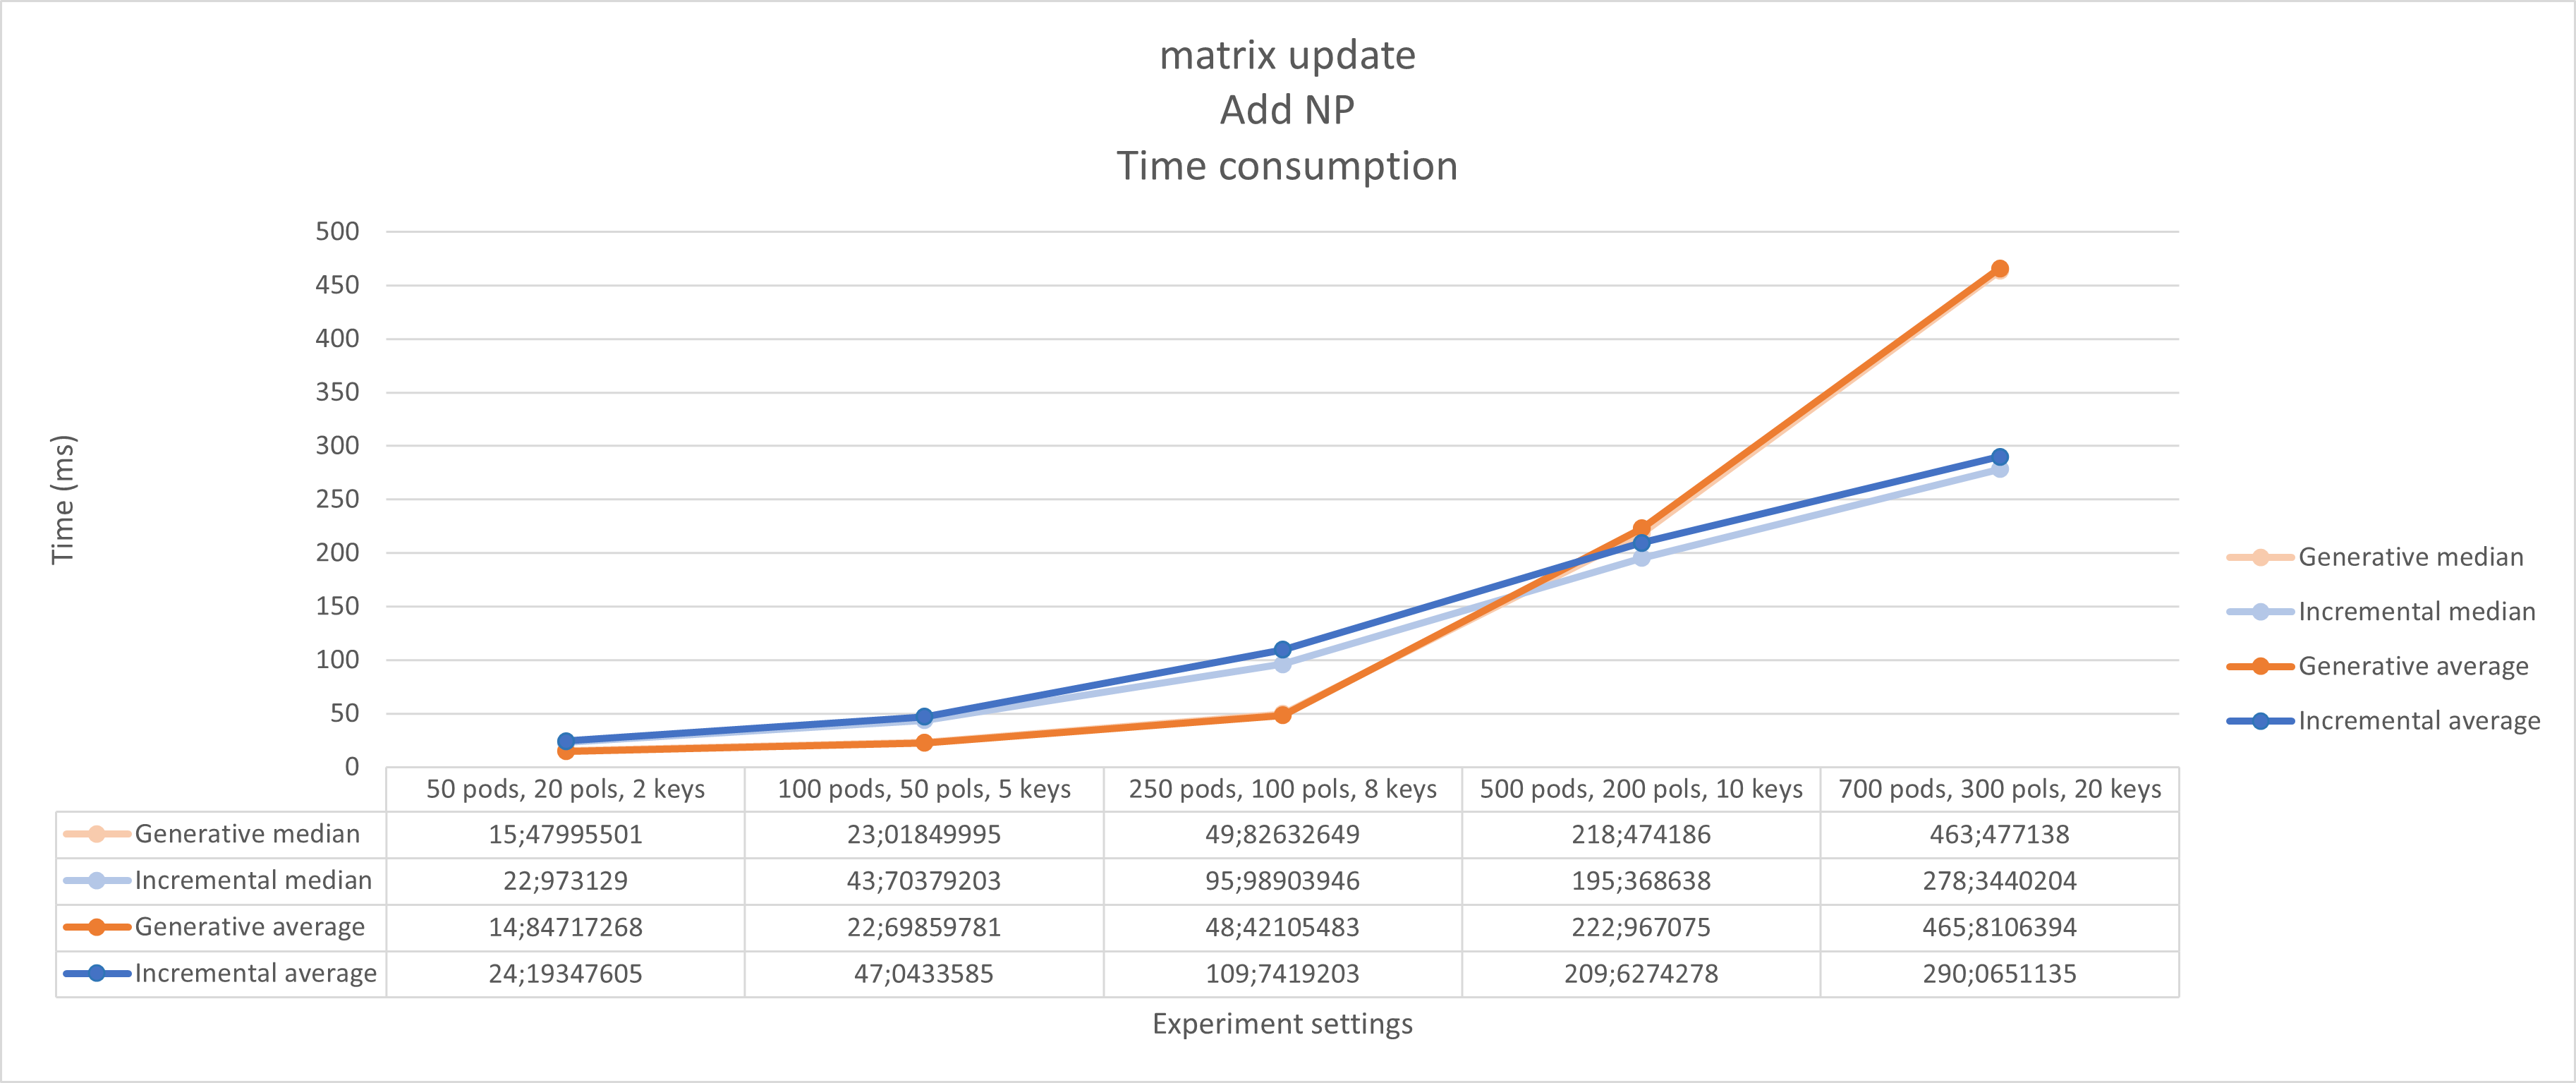
\includegraphics[width=\textwidth]{images/experiment1/addNP-time.png}
    \caption{Time consumption of adding a network policy}
    \label{fig:exp1-addNP-time}
\end{figure}
\begin{figure}[H]
    \centering
    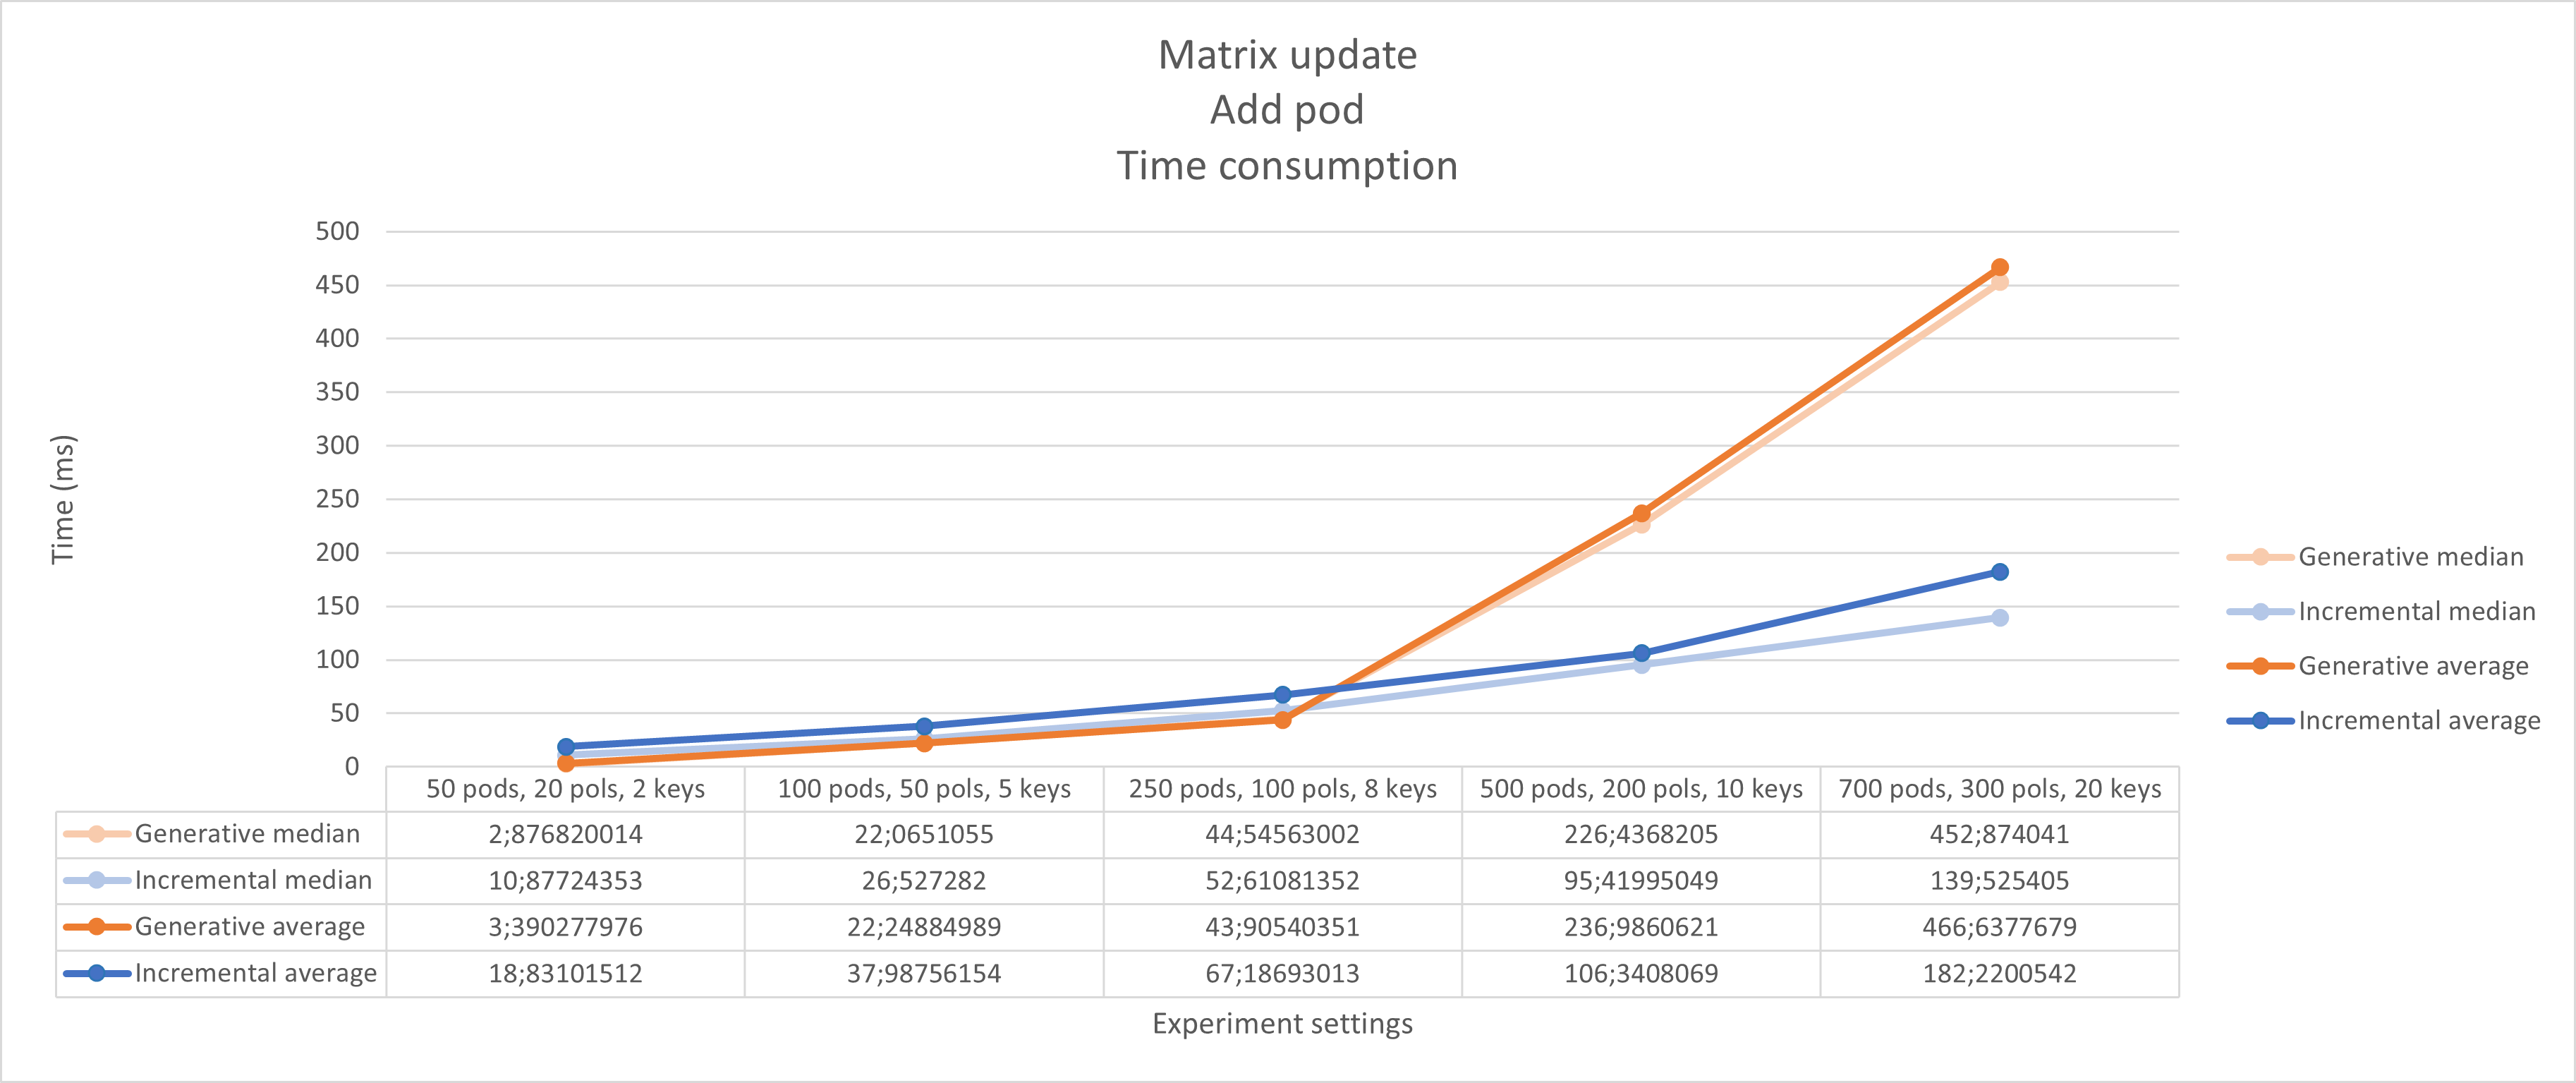
\includegraphics[width=\textwidth]{images/experiment1/addPod-time.png}
    \caption{Time consumption of adding a container}
    \label{fig:exp1-addPod-time}
\end{figure}
\begin{figure}[H]
    \centering
    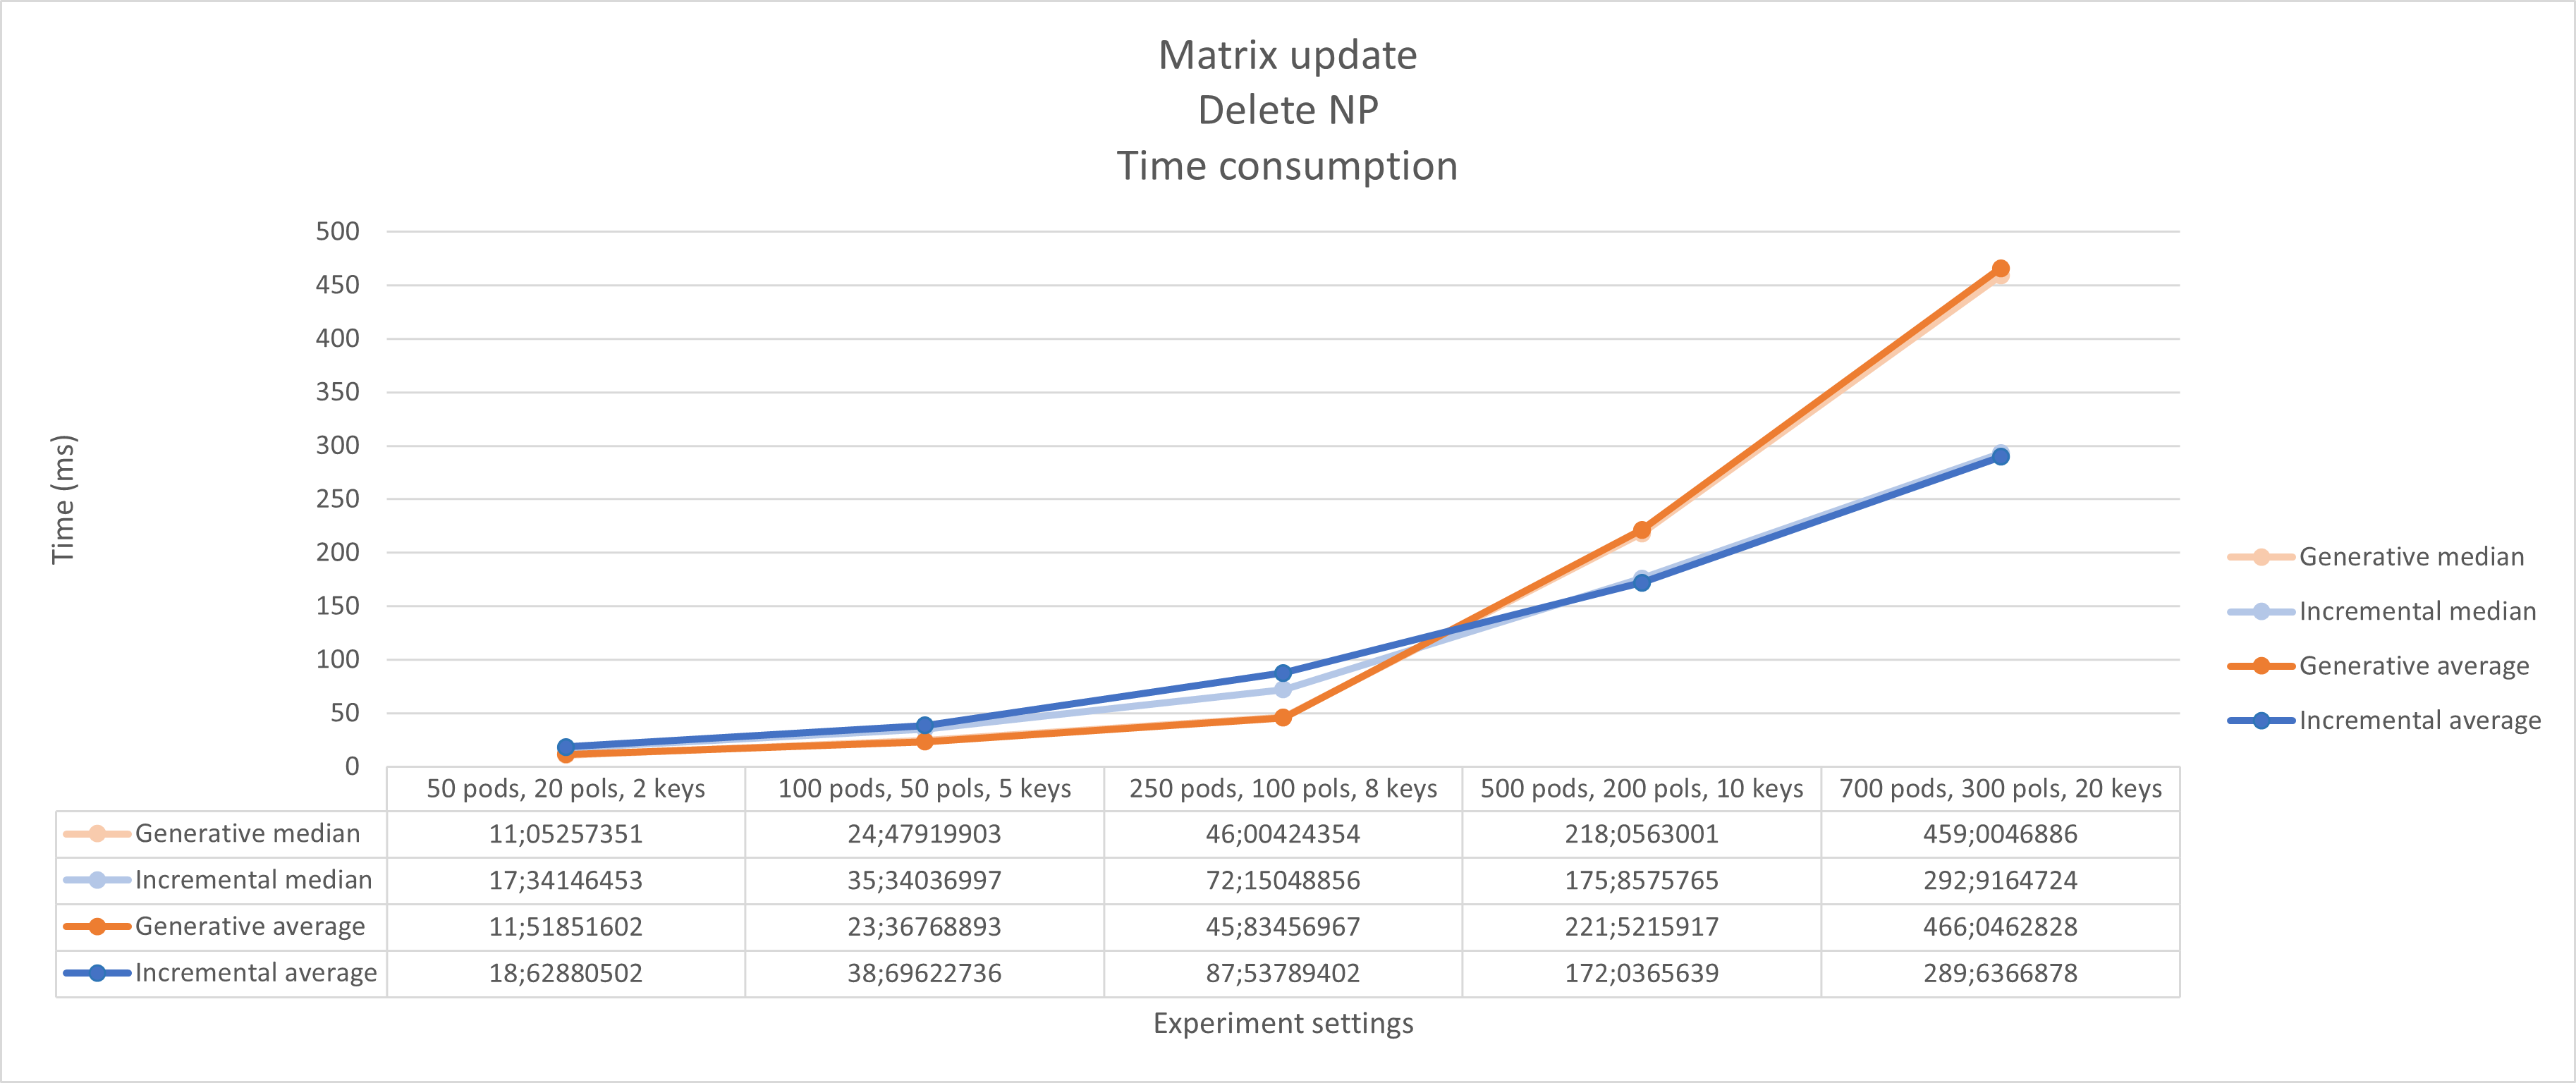
\includegraphics[width=\textwidth]{images/experiment1/delNP-time.png}
    \caption{Time consumption of deleting a network policy}
    \label{fig:exp1-delNP-time}
\end{figure}
\begin{figure}[H]
    \centering
    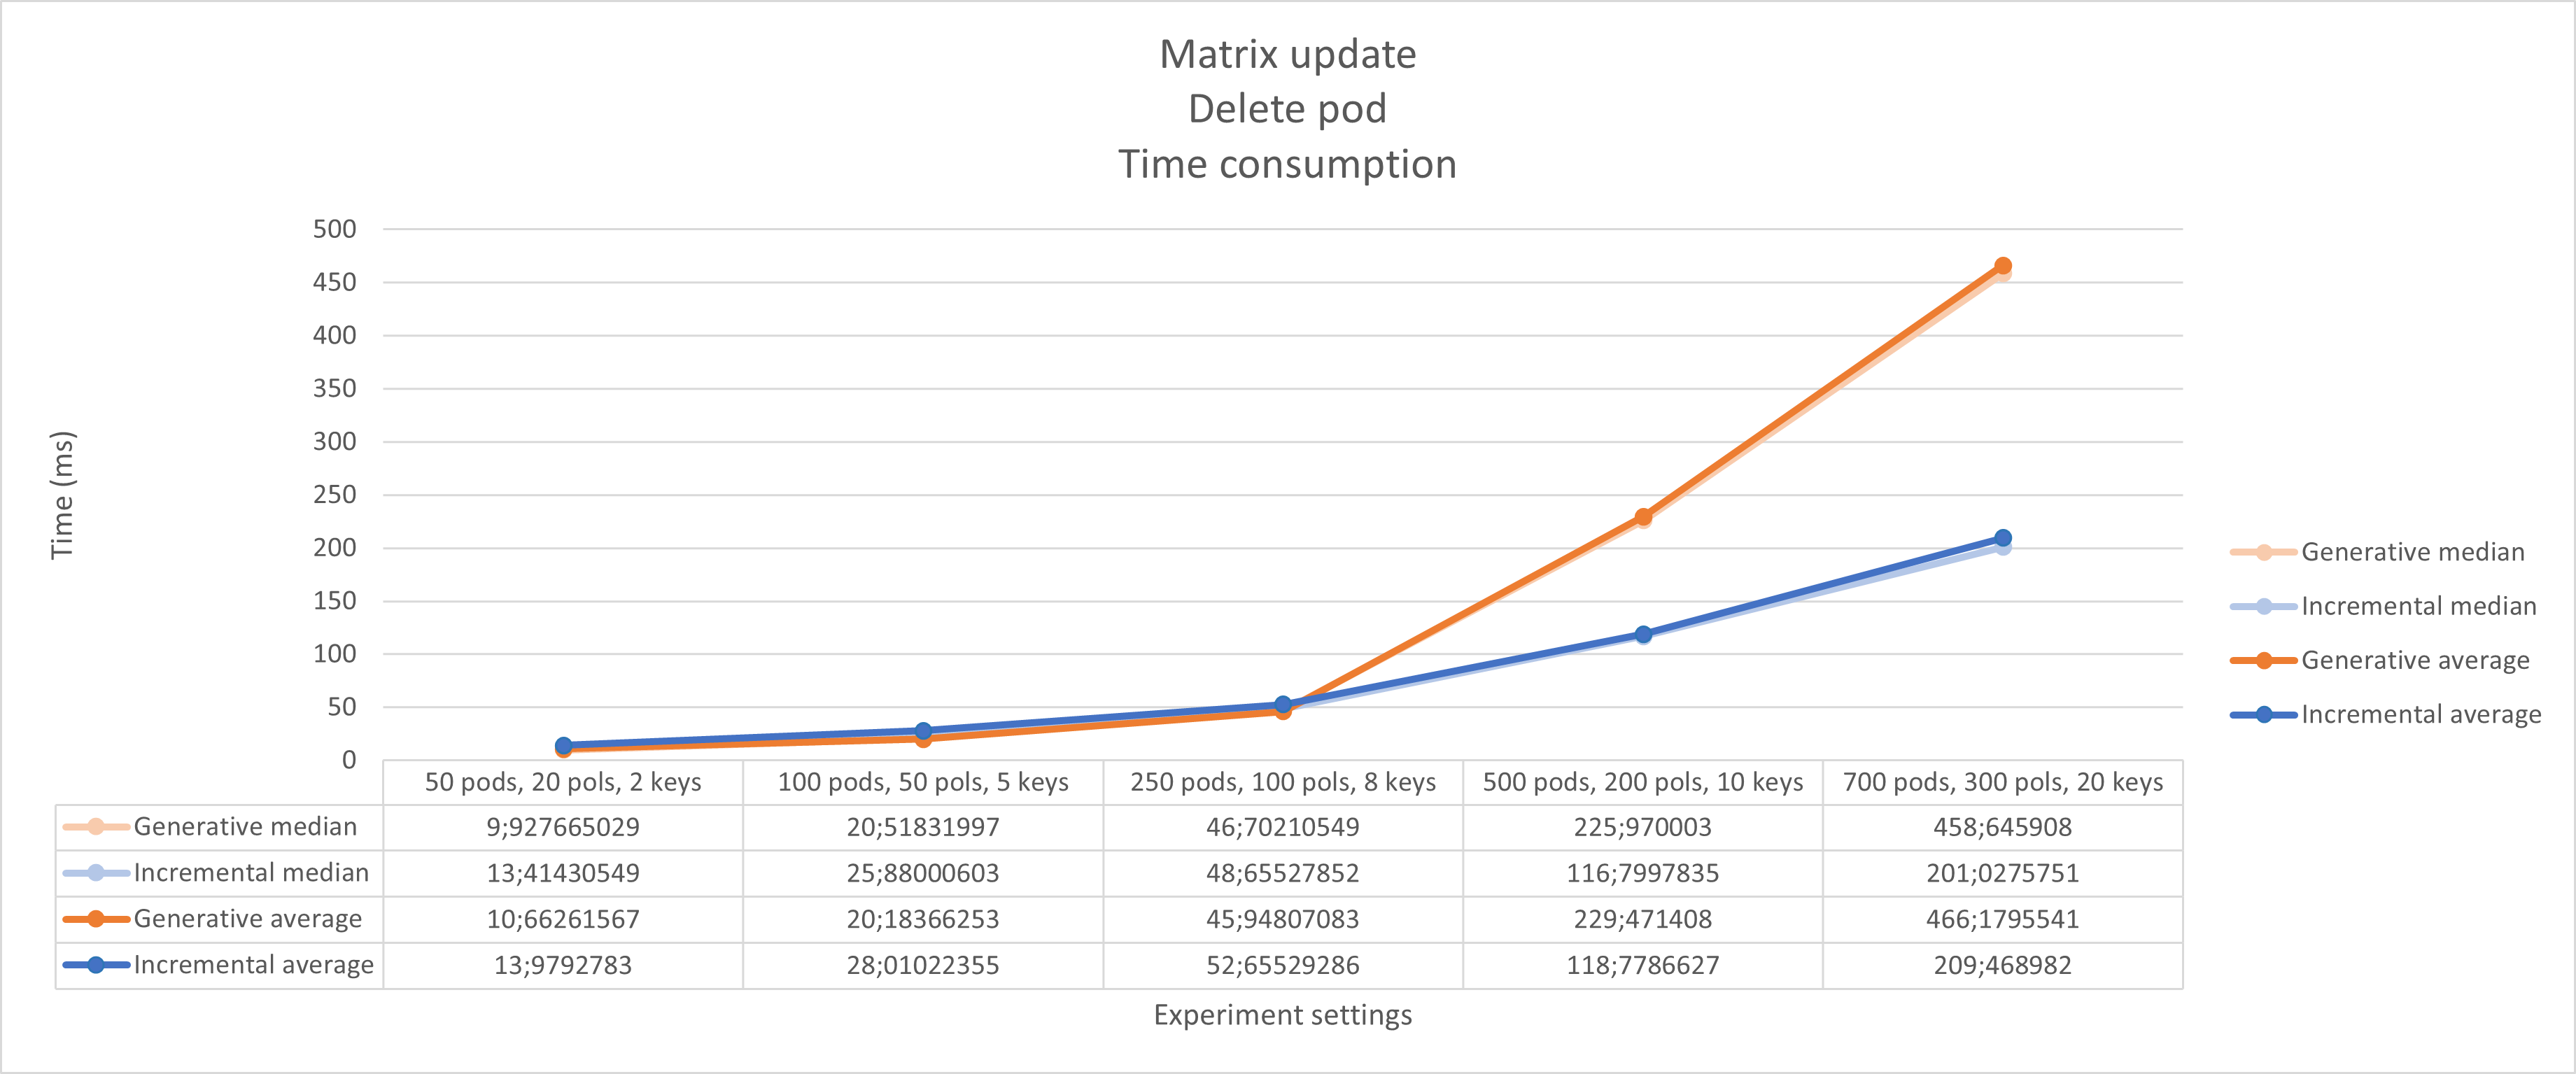
\includegraphics[width=\textwidth]{images/experiment1/delPod-time.png}
    \caption{Time consumption of deleting a container}
    \label{fig:exp1-delPod-time}
\end{figure}



\textbf{Memory consumption}
\newline When looking at the graphs in \autoref{fig:exp1-addNP-memory}, \autoref{fig:exp1-addPod-memory}, \autoref{fig:exp1-delNP-memory}  and \autoref{fig:exp1-delPod-memory} we can quickly deduce that our incremental approach is more expensive in terms of memory usage than the generative approach, with the difference only increasing as the cluster grows. This is in line with our expectation for Q2 described in \autoref{sec:experiment1}. Next, we present some additional observations we can deduce from these graphs:
\begin{itemize}
    \item With a small exception for the fifth sub-experiment in the creation event of a network policy, the median values are almost identical to the average values, meaning little skewing of data between the runs occurs. This makes sense since the cluster state that we store always has the same amount of cluster objects to keep track of within each run. The exception mentioned before might be due to a high occurrence of matching labels between objects which in turn increases the size of data structures such as the Store keeping track of \acrshort{np}s responsible for connections between pods. However, this remains an educated guess at best.
    \item We can see that the ratio in which the memory increases for the incremental method decreases slightly between the fourth and fifth sub-experiments. We have no direct explanation for this, and further research would be necessary to deduct more from this. 
 	\item Although the incremental approach has higher memory consumption it should be noted that the generative approach can not be used in its current form to execute conflict detection and would need adaptations to store more information. We can therefore not conclude that our incremental approach is strictly worse in terms of memory consumption than the generative approach.
\end{itemize}

\begin{figure}[H]
    \centering
    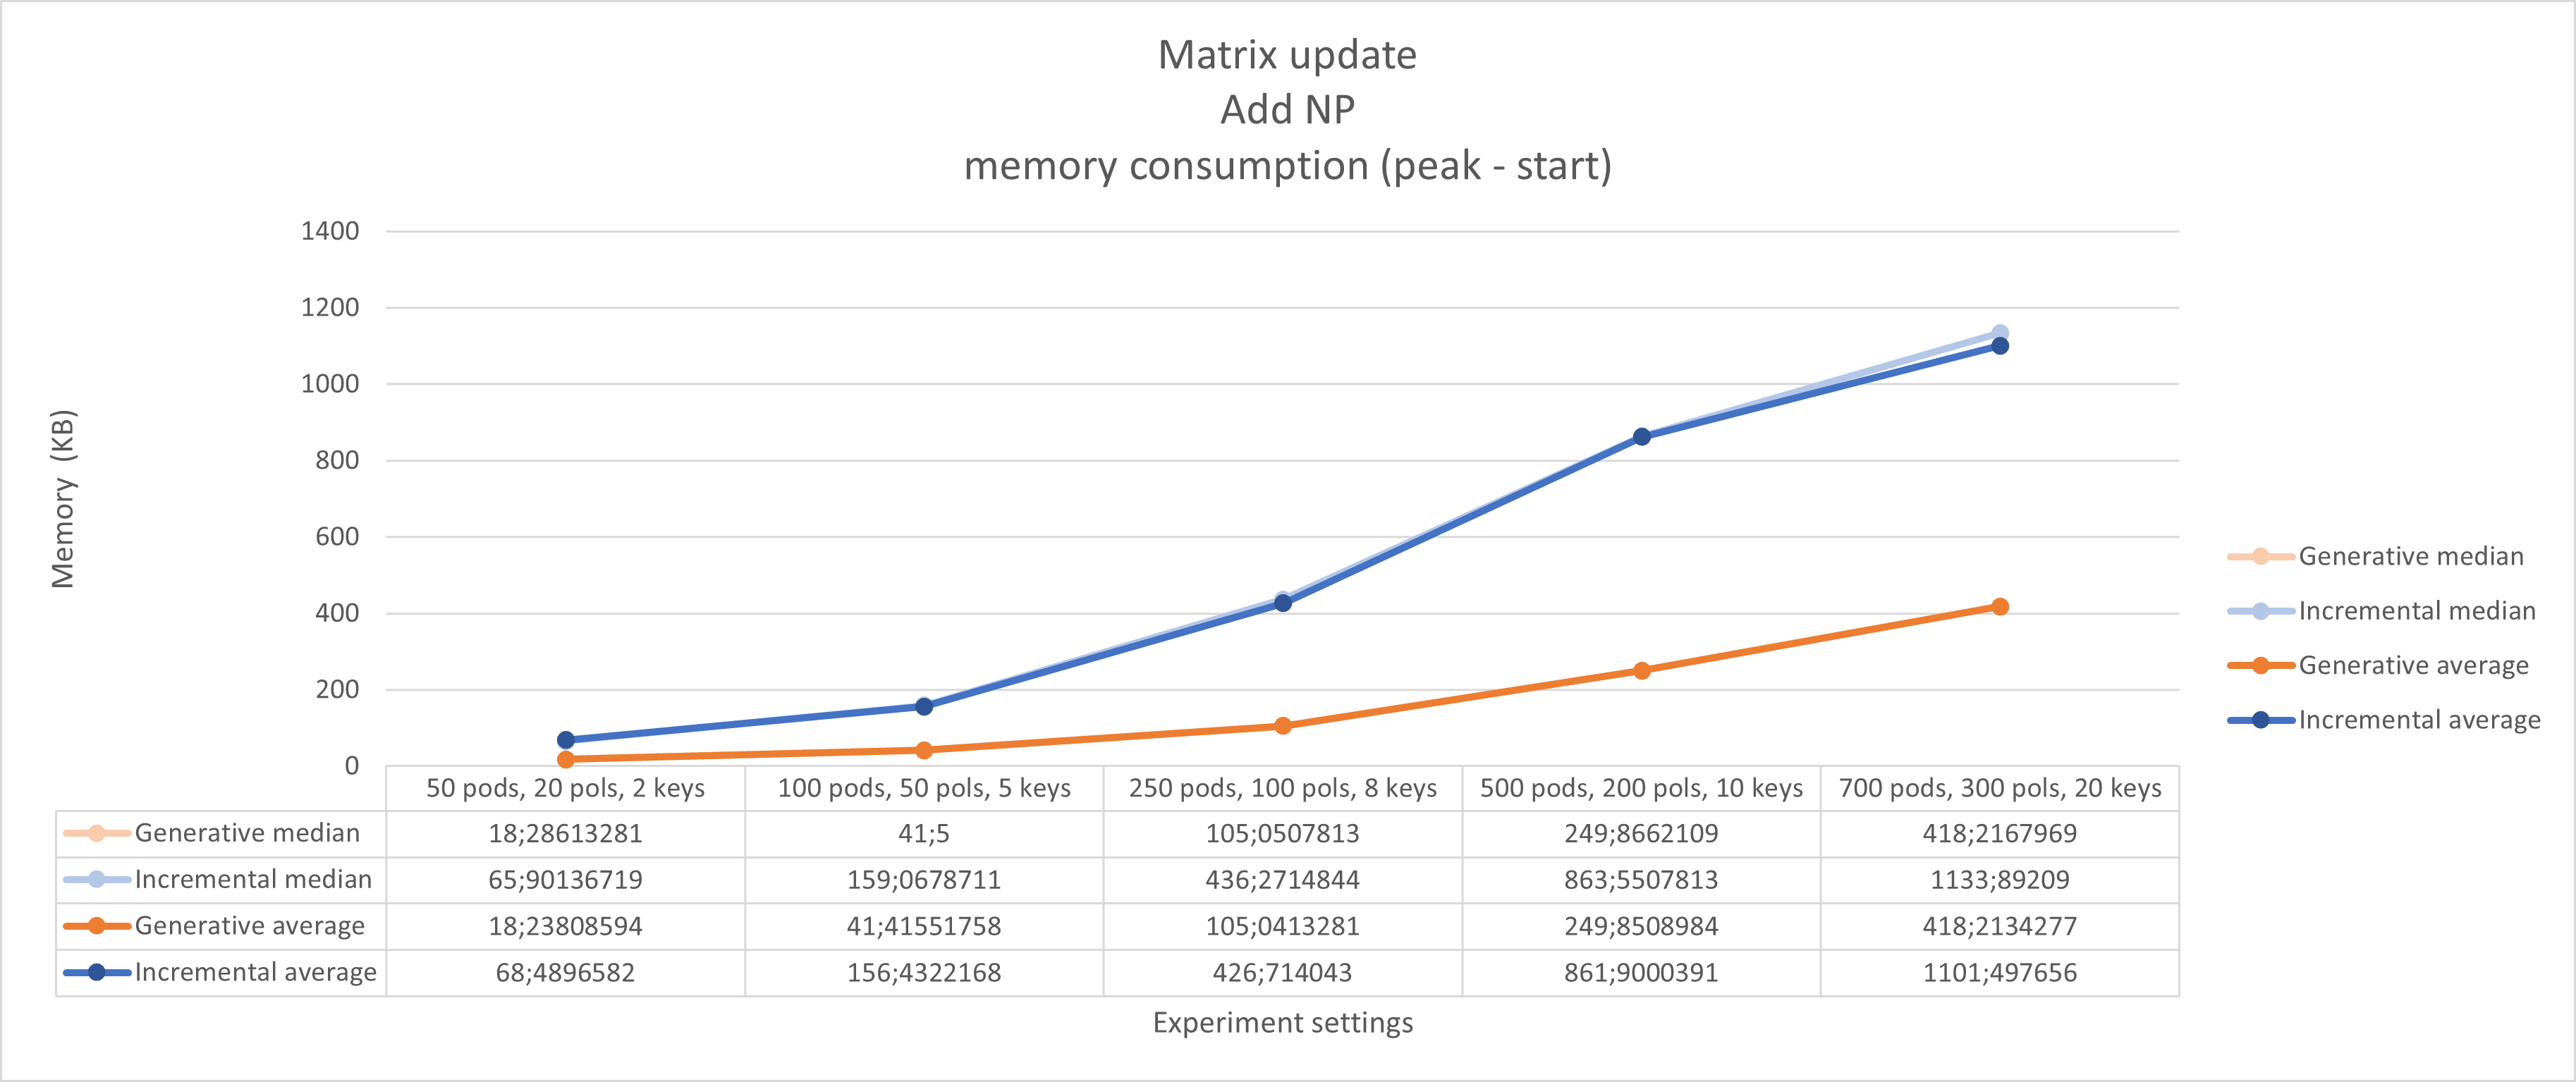
\includegraphics[width=\textwidth]{images/experiment1/addNP-memory.png}
    \caption{Memory consumption of adding a network policy}
    \label{fig:exp1-addNP-memory}
\end{figure}
\begin{figure}[H]
    \centering
    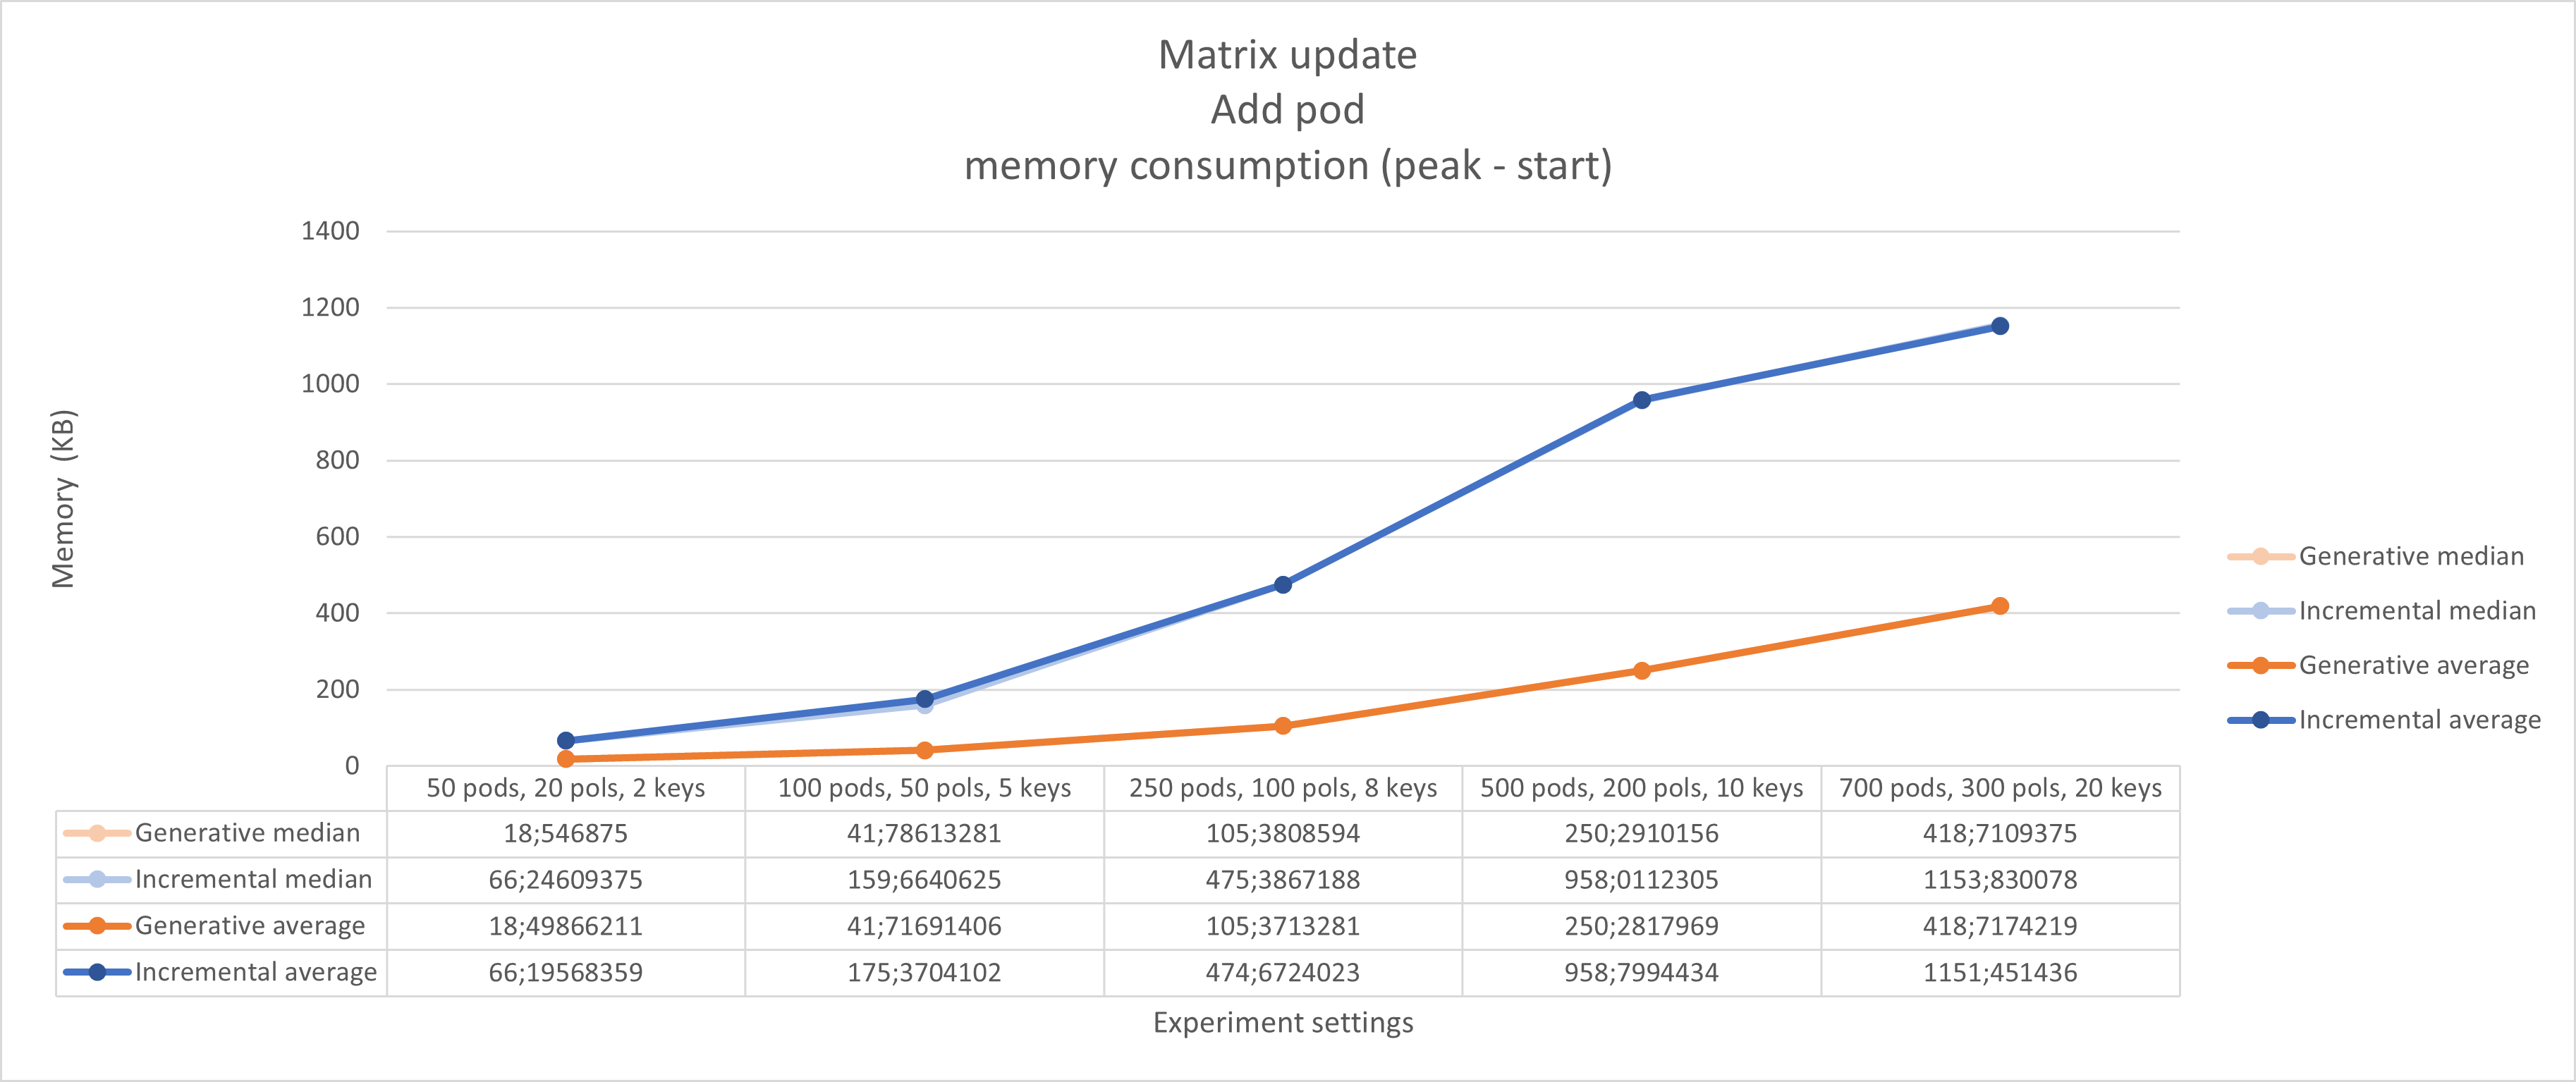
\includegraphics[width=\textwidth]{images/experiment1/addPod-memory.png}
    \caption{Memory consumption of adding a container}
    \label{fig:exp1-addPod-memory}
\end{figure}
\begin{figure}[H]
    \centering
    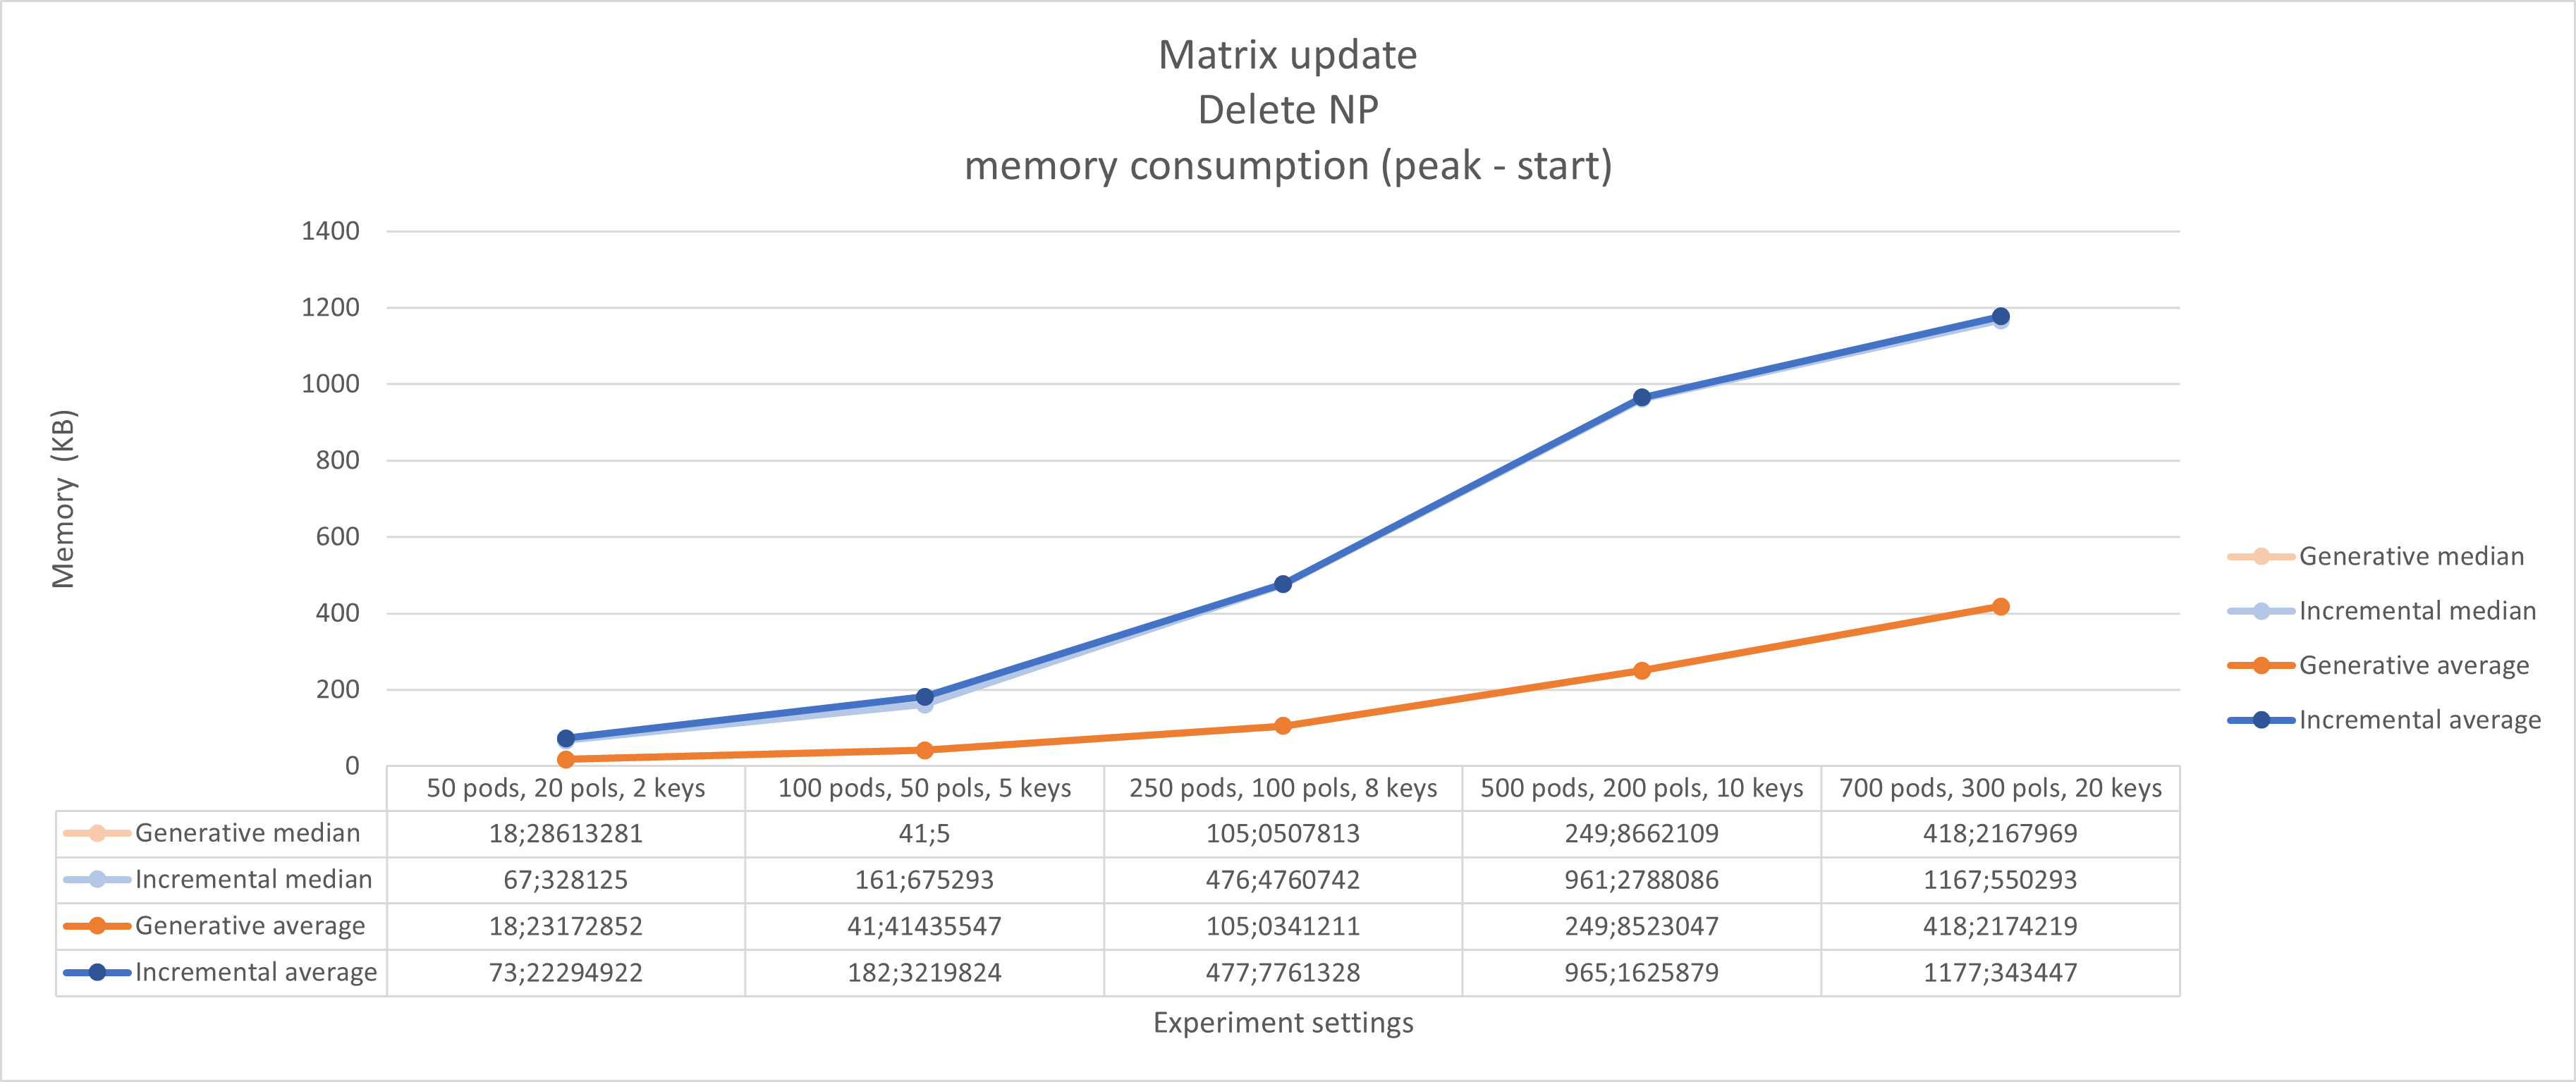
\includegraphics[width=\textwidth]{images/experiment1/delNP-memory.png}
    \caption{Memory consumption of deleting a network policy}
    \label{fig:exp1-delNP-memory}
\end{figure}
\begin{figure}[H]
    \centering
    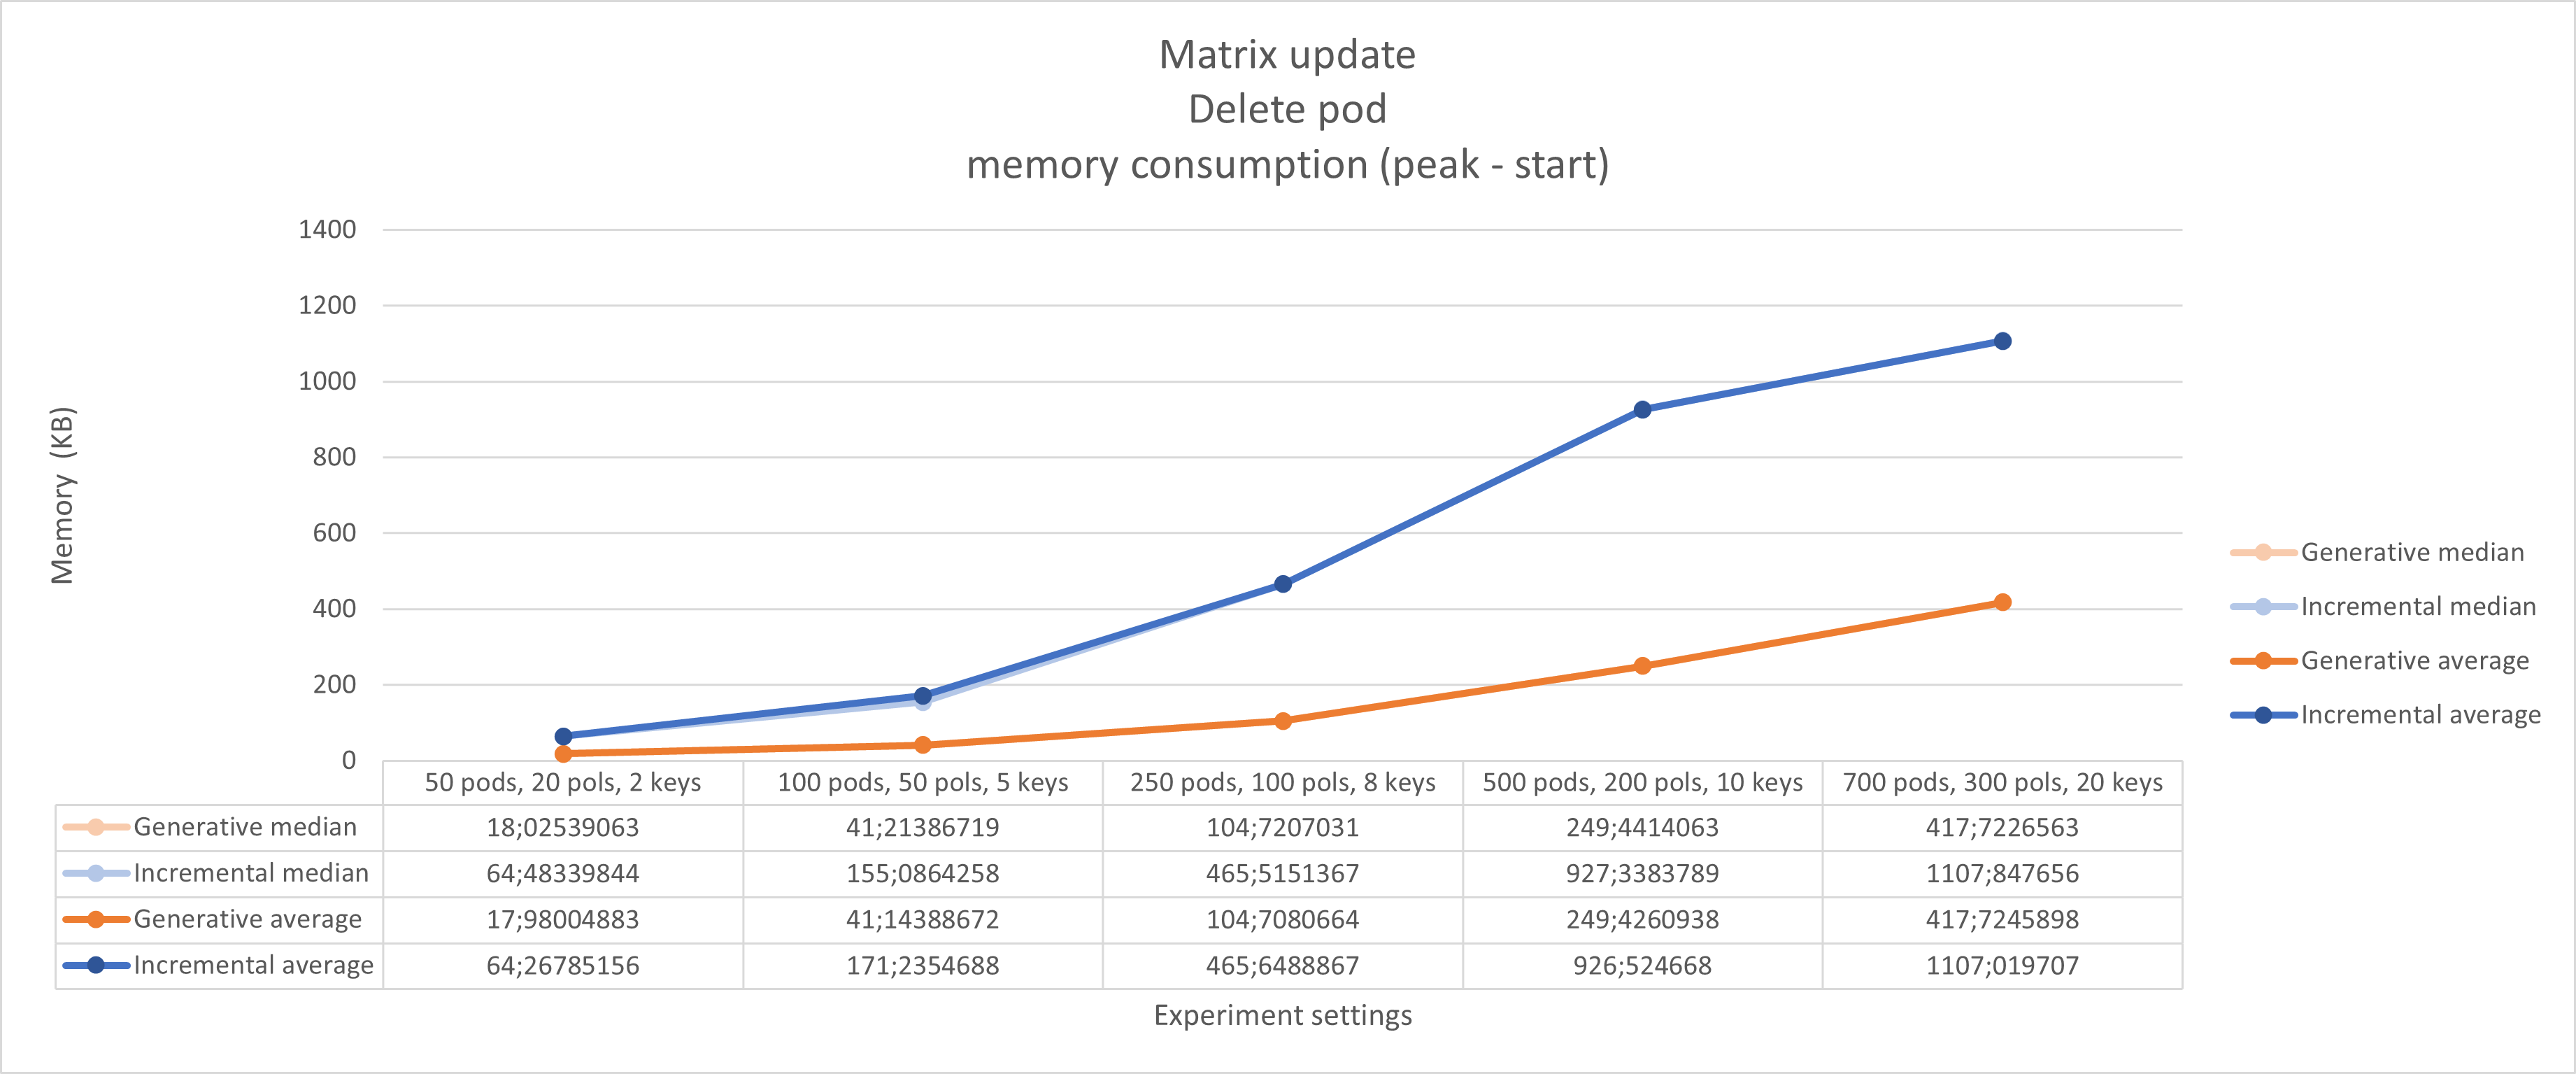
\includegraphics[width=\textwidth]{images/experiment1/delPod-memory.png}
    \caption{Memory consumption of deleting a container}
    \label{fig:exp1-delPod-memory}
\end{figure}



% ========================================================================================
\section{Experiment 2}\label{sec:experiment2}
The second experiment aims to give more insight into the overhead created by running our complete conflict detection algorithm on a cluster and will answer the following research questions:

\begin{itemize}
    \item \textit{Q3:} What is the relationship between pod/policy numbers and the time cost of conflict detection?
    \item \textit{Q4:} What is the relationship between pod/policy numbers and the space cost of conflict detection?
\end{itemize}

Before we delve into the experiment approach, setup and results we declare our expectations for the experiment:

\begin{itemize}
    \item \textit{Expectation E3:} We expect that the time that the algorithm takes will be less than 50\% of the average deployment time* of a pod, but that the time cost of our algorithm will increase as the cluster size increases. 
    \item \textit{Expectation E4:} We expect that the space cost of our algorithm will increase as the number of pods and \acrshort{np}s in the cluster increases as well. 
\end{itemize}

* In the research paper of Grasshopper they found that during their experiments the deployment time of an application can be up to 4 seconds in case of a cold start \cite{grashopper}. Since there is no default redeployment time for a container in a \acrshort{k8s} cluster we use this as a baseline. Note that an estimate for conflict detection and resolution can be found by adding the time usage of our algorithm and a cold start deployment together.

% =========================================
\subsection{Approach} \label{exp2:approach}
For this experiment, we must use the entire algorithm instead of using a smaller part as we did in experiment 1. We can not compare our conflict detection, however, since there is no other research solution that provides the same functionality to the best of our knowledge. Instead, we measure general information about time and memory consumption when handling events. We once again use the same experiment setups as used in experiment 1 but must define additional parameters for the generation of the security groups and security group rules in the \acrshort{sgic} component. We will now describe the meaning of these additional parameters, while their values for this experiment can be seen in \autoref{tab:exp2pars}.

\begin{itemize}
    \item \textit{Nr of SG}: This constant describes the minimum and maximum amount of security groups that will be generated when initializing the \acrshort{sgic}. The exact amount of security groups are thus randomly selected between these values.
    \item \textit{Nr of SG rules }: This constant describes the minimum and maximum amount of security group rules that will be generated for each security group when initializing the \acrshort{sgic}. The exact amount of security group rules per security group is thus randomly selected between these values.
    \item \textit{Nr of SG linked to node}: This constant describes the minimum and maximum amount of security groups that will be linked to a node. The exact amount of linked security groups is thus randomly selected between these values and is different for each node.
\end{itemize}

Lastly, we would like to mention that the variables within the security groups and security group rules are randomised as well. There is a 3\slash 5 chance that a security group rule applies to a security group and a 2\slash 5 chance that it will specify an IP address. These IP addresses are randomised between 10 different values out of which 7 are the IPS of the nodes on the cluster to increase the chance of matching rules. 


\begin{table}[H]
    \centering
    \begin{tabular}{|l|c|c|c|c|c|}
        \hline
        \textbf{Name} & \textbf{setup 1} & \textbf{setup 2} & \textbf{setup 3} & \textbf{setup 4} & \textbf{setup 5}\\
        \hline
        Pod num & 50 & 100 & 250 & 500 & 750 \\
        Pol num & 20 & 50 & 100 & 200 & 300 \\
        Key limit & 2 & 5 & 8 & 10 & 20 \\
        Value limit & 10 & 10 & 10 & 10 & 10 \\
        Pol select limit & 1 & 1 & 1 & 1 & 1 \\
        Pol select label limit & 3 & 3 & 3 & 3 & 3 \\
        Pol allow limit & 3 & 3 & 3 & 3 & 3 \\
        Pol allow label limit & 3 & 3 & 3 & 3 & 3 \\
        Pod label limit & 5 & 5 & 5 & 5 & 5 \\
        Nr of SG & 6-16 & 6-16 & 6-16 & 6-16 & 6-16\\
        Nr of SG rules & 3-5 &3-5 & 3-5 & 3-5 & 3-5\\
        Nr of SG linked to node & 3-5 &3-5 & 3-5 & 3-5 & 3-5\\
	
        \hline
    \end{tabular}
    \caption{Experiment 2 parameter values}
    \label{tab:exp2pars}
\end{table}

The measurements retrieved from this experiment can be split into two parts: we analyze how long it takes for the watcher to get fully initialised and ready for capturing events, while also measuring the time and memory cost of our entire conflict detection algorithm in specific scenarios. For the first part of the experiment, we only retrieve the time between calling the watcher and it returning the ready status (ms). The second part is more extensive as we collect the time between applying an event and detection by the watcher (ms), the time it takes for conflict detection (ms) and lastly, the total time which is the combination of these last two (ms). 

% =========================================
\subsection{Execution} \label{exp2:execution}
The approach for this experiment is very similar to experiment 1 but with small yet very important changes.  We will now describe the execution of a single sub-experiment step by step where we will highlight the changes made in comparison with experiment 1.
\\[10pt]

\textbf{STEP 0:} Call the python file experiment2.py with the following arguments: $number\_of\_runs$, $number\_of\_pods$, $number\_of\_policies$, $namespace$, $key\_limit$ and $event\_type$ according to the sub-experiment settings. The algorithm will then execute STEP 1 to STEP 7 as many times as defined in argument $number\_of\_runs$.
\\[10pt]

\textbf{STEP 1:} We fully reset the namespace defined in the $namespace$ argument with the help of the Python \acrshort{k8s} API. This is coded in a separate delete.py file and extended with some extra tests and timeouts to guarantee that all objects are successfully removed before continuing.
\\[10pt]

\textbf{STEP 2:} We deploy as many pods and \acrshort{np}s as defined in arguments \newline $number\_of\_pods$ and $number\_of\_policies$. For this functionality a separate deploy.py python file has been created that will generate and deploy the \acrshort{np}s and pods, when called upon with the variables $namespace$ and $key\_limit$ as parameters. The other relevant constants in \autoref{tab:exp2pars} are hard coded since they don't change between sub-experiments. The deploy file is equipped with a list of distinct keys and values to leverage when creating the randomised pods and \acrshort{np}s. However, the key list is first shortened until it has a length equal to the $key\_limit$ parameter before being utilised. The randomised pods and \acrshort{np}s get deployed in the namespace defined in the $namespace$ argument with the help of the Python \acrshort{k8s} API. We use extra tests and timeouts to guarantee all objects are successfully deployed and ready before continuing. 
\textbf{We retrieve and store the current time and start the memory tracer}.
\\[10pt]

\textbf{STEP 3:} We start the watcher with the flags for debug mode,  verbose mode and start the checkup all set to False. With the use of threading events, we guarantee that the threads that watch the APIs for pods and \acrshort{np}s are successfully running, in order to prevent the next step from executing too early, therefore missing the event and being unable to handle it. \textbf{When the watcher returns that it is ready and monitoring the cluster we save the time and stop the memory tracer to store these for later evaluation}.
\\[10pt]

\textbf{STEP 4:} We execute one event, depending on the $event\_type$ argument. If it is a delete event we call the delete.py file again and let it randomly remove one of the existing objects that correspond to the event type. If it is a deploy event we call the deploy.py file to generate one more randomly generated object according to the correct parameters. \textbf{We save the time at which we send the API request to the \acrshort{k8s} API server}.
\\[10pt]

\textbf{STEP 5:} We once again leverage threading events to get notified when the consumer thread has received and handled its first event. Since the watcher was initialized after all pods and \acrshort{np}s were fully ready it will always be the event from step 4 that will be caught. When the consumer catches the event it will start the timer right before calling the analyzer for event handling. Once the analyzer returns the function call the timer immediately gets stopped to get a final execution time. Similarly, we measure the memory usage at the start of the algorithm, and the highest peak of memory usage during the event handling. With this we can calculate the difference and thus how much memory was used (in bytes). These memory and time measurements get stored in variables in the watcher.
\\[10pt]

\textbf{STEP 6:} Once we get the message that the event is handled we retrieve the measurements from the watcher and store it locally. We can then stop the watcher. 
\textbf{This includes the time at which the event was detected by the watcher.} \textbf{With all the time measurements that we collected we calculate some usable values such as the time between the \acrshort{k8s} API call and event detection, and the total time between the \acrshort{k8s} API call and completion of conflict detection}.
\\[10pt]

\textbf{STEP 7:} Once the hundred runs of the sub-experiment have finished we store all the data in a CSV file and store it on the control plane node that ran the experiment. We can then retrieve this file and combine it with other sub-experiment files for evaluation.  \textbf{Since there is no comparison in experiment 2 step 7 equals to step 8 of experiment 1}. 
\\[10pt]


% =========================================
\subsection{Experiment results} \label{exp2:results}
Similarly to experiment 1 we created two graphs for each of the four captured events: one for the average and median time and the other for the average and median memory consumption. When comparing the graphs with experiment 1 we can see that there are only two data lines instead of four since there is only a single update method of the reachabilitymatrix used. Additionally, the graphs show data for the entire conflict detection solution instead of solely the update of the reachabilitymatrix. Aside from these 8 event graphs we also have two graphs regarding the time and memory consumption of the startup process of the watcher which is defined as the period between execution of the script up until the point at which the algorithm is readily monitoring the cluster. This startup data thus includes initialization of variables, reachabilitymatrix generation, cloud layer generation and setting up multithreaded API monitors. In these startup graphs, we do not separate the data per event since the event has not occurred yet when the algorithm is initialized and thus has no influence. Please note that the conflict detection graphs all use the same values and increments on their axis to allow a direct comparison, but the startup graph does not follow this promise: it shows the time in seconds instead of milliseconds. We will start by looking at the startup graphs after which we continue with the time and memory graphs for conflict detection.
\\[10pt]

\textbf{Watcher Startup}
\newline The time and memory consumption for initialising the watcher can be seen in \autoref{fig:exp2-startup-time} and \autoref{fig:exp2-startup-memory} respectively. The goal of these graphs is to give a general sense of resource consumption for the algorithm's startup phase, but we have no hard time limit imposed since the algorithm should in theory only be started once, and usually in a non-time-sensitive environment. We can deduct two interesting conclusions from the graphs:

\begin{itemize}
    	\item The median time deviates from the average time, which we attribute once again to the idea that the amount of connections in the cluster setup directly influences the speed of our solution. This difference increases with cluster size since more \acrshort{np}s and containers directly translate to a higher chance of container connection.
	\item The memory consumption shows no surprises nor does it show any significant difference between the average and mean values, indicating that our algorithm remains very stable. Interestingly enough this indicates that variables whose size depends on the number of allowed connections, such as resp\_policies  in the reachability structure (see \autoref{impl:model}) do not have much influence on the total memory consumption.

\end{itemize}

\begin{figure}[H]
    \centering
    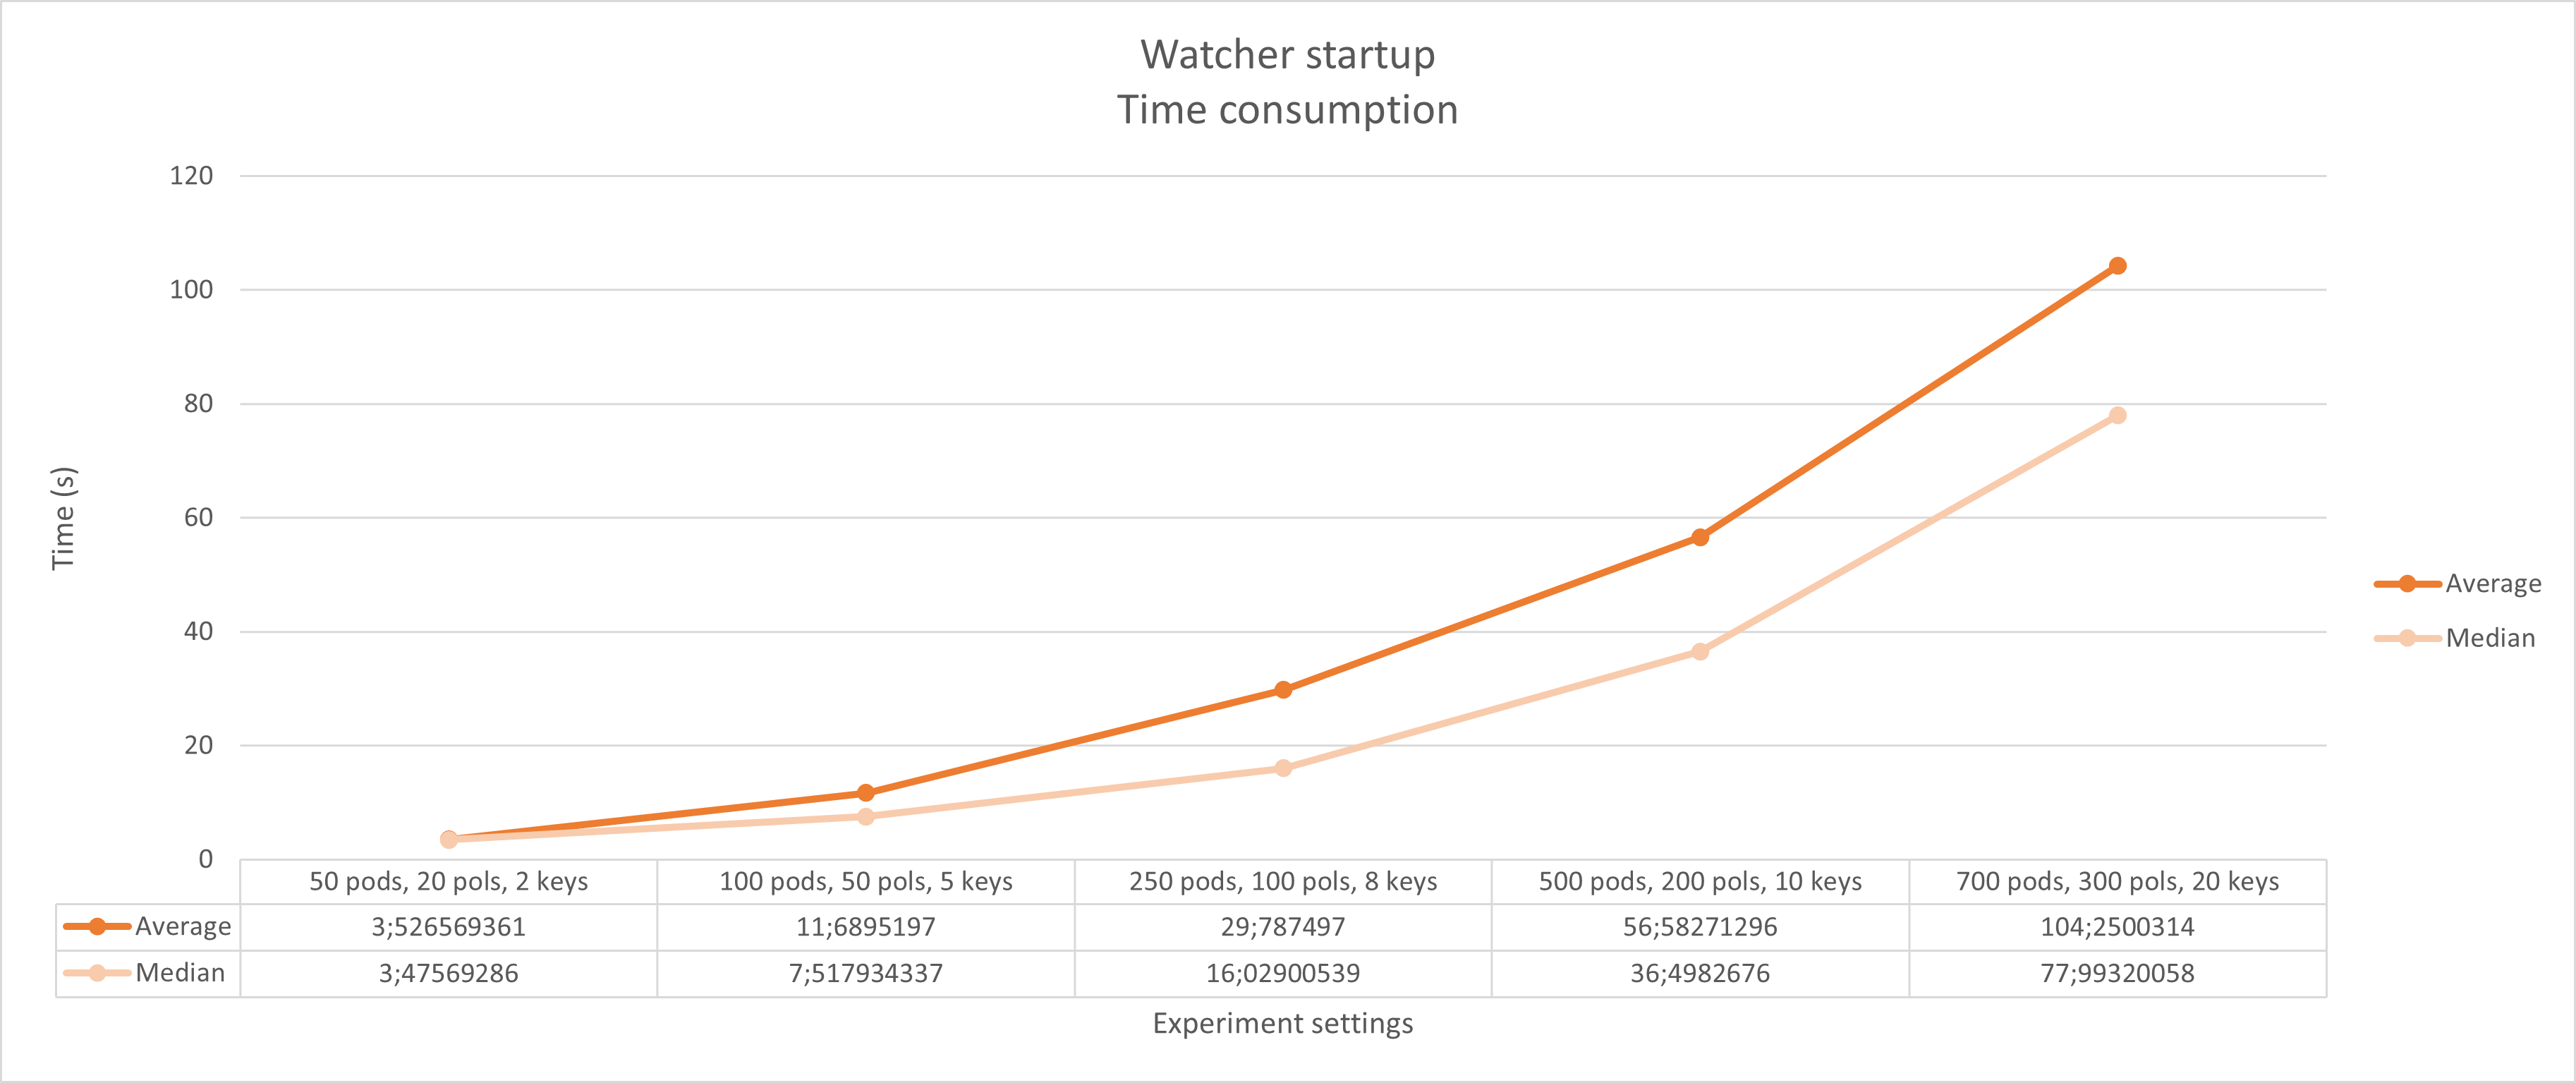
\includegraphics[width=\textwidth]{images/experiment2/watcher-startup-time.png}
    \caption{Time consumption of starting up the algorithm}
    \label{fig:exp2-startup-time}
\end{figure}
\begin{figure}[H]
    \centering
    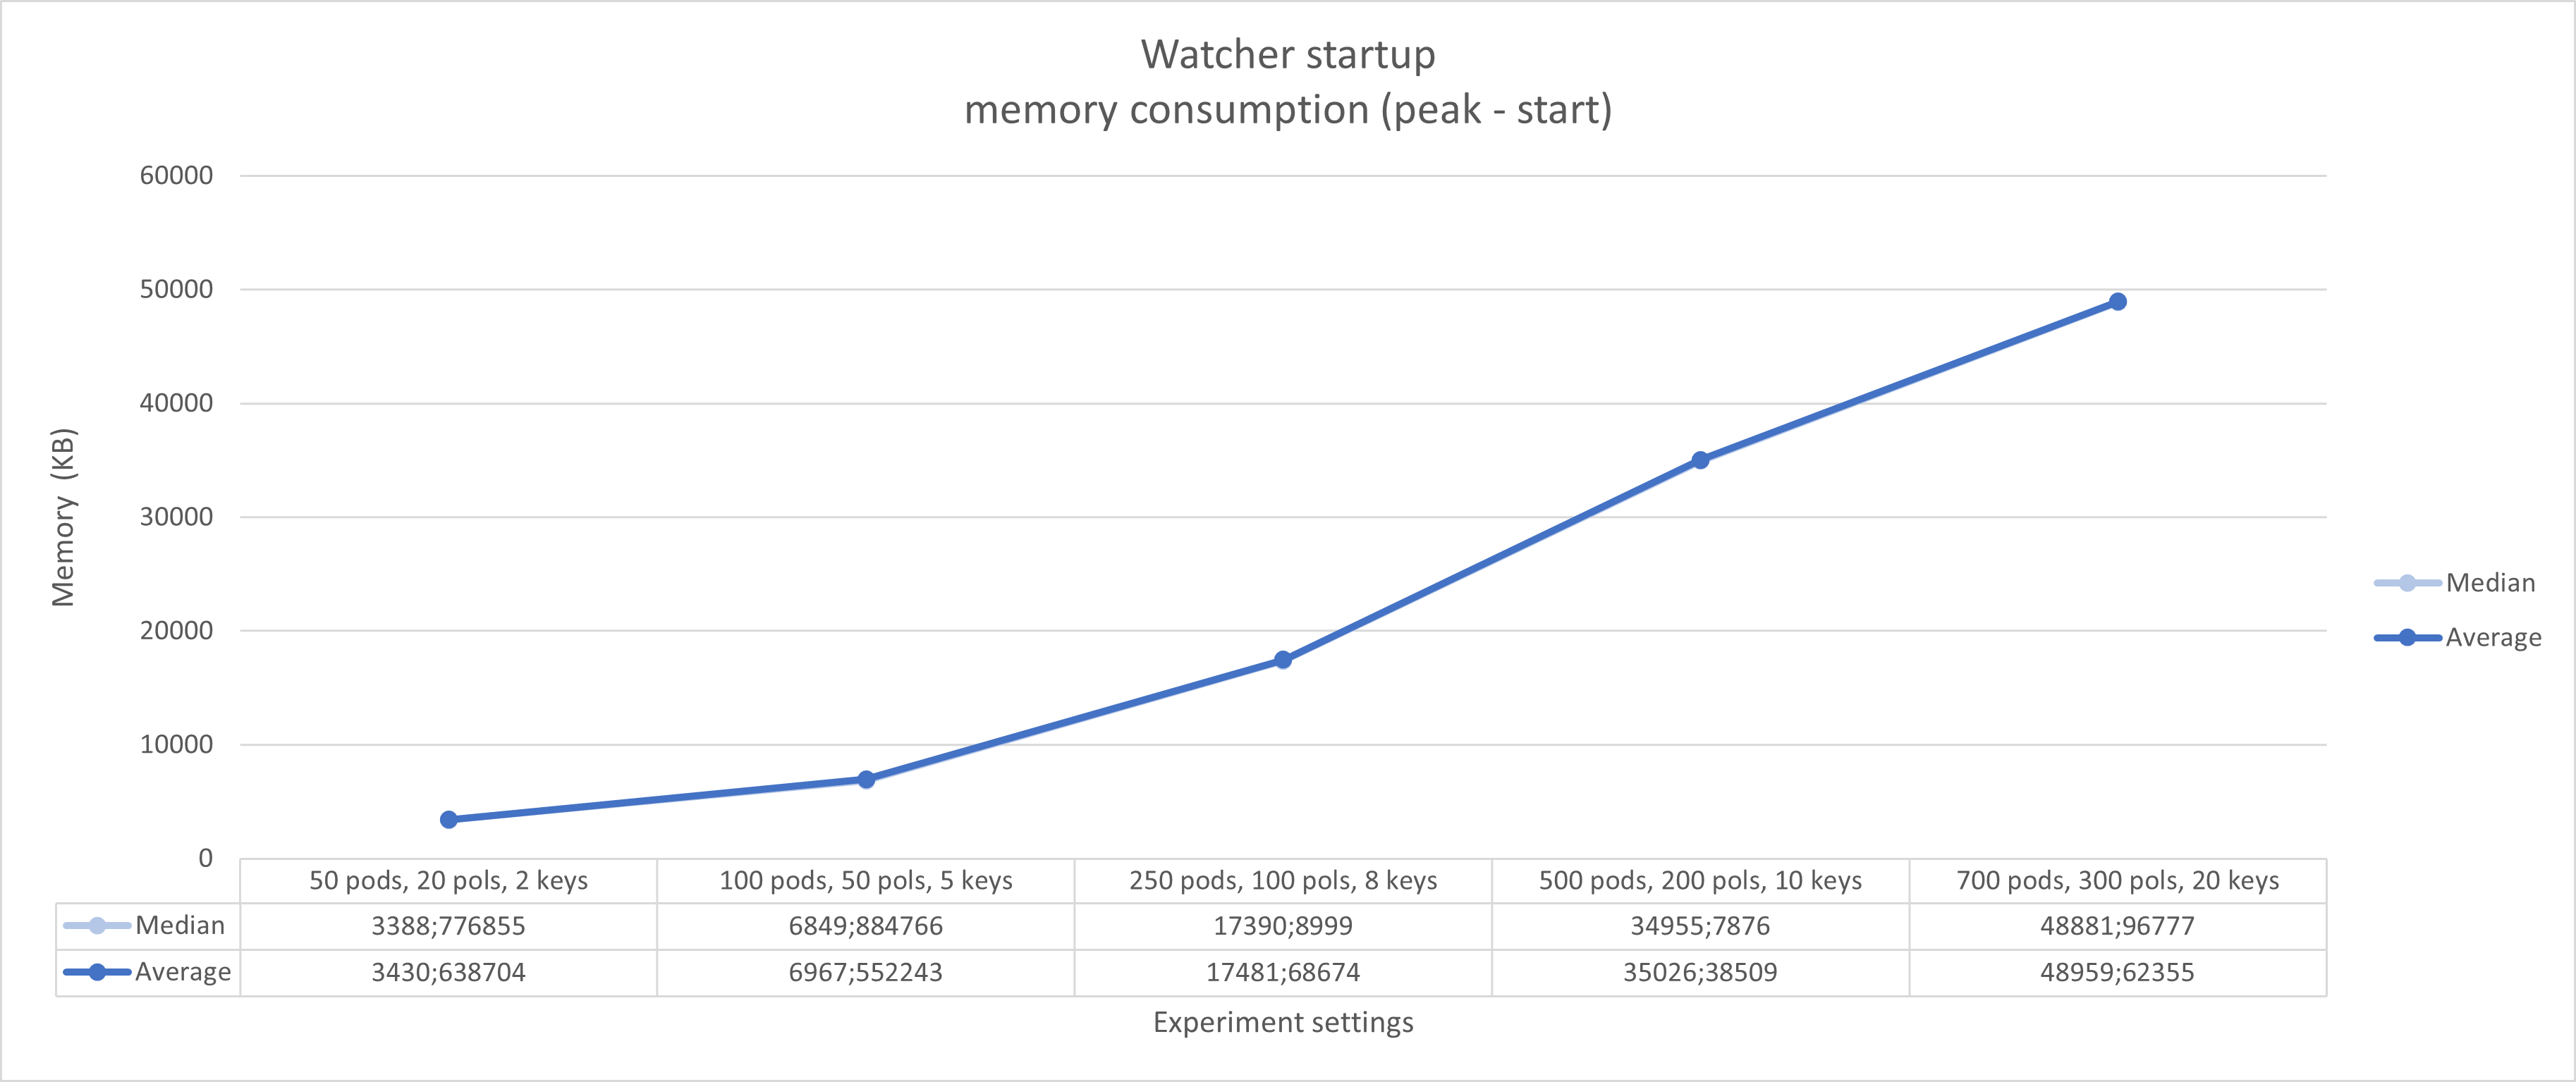
\includegraphics[width=\textwidth]{images/experiment2/watcher-startup-memory.png}
    \caption{Memory consumption of starting up the algorithm}
    \label{fig:exp2-startup-memory}
\end{figure}



\textbf{Time consumption}
\newline The time consumption for the full conflict detection solution for each of the four events are shown in \autoref{fig:exp2-addNP-time-conflict}, \autoref{fig:exp2-addPod-time-conflict}, \autoref{fig:exp2-delNP-time-conflict} and \autoref{fig:exp2-delPod-time-conflict}.  We can see that the conflict detection time remains safely below the 4-second pod deployment threshold stated in the expectation for Q3 with the highest average being 474ms for the deletion of a network policy. Furthermore, we can deduct some interesting information from the graphs:
\begin{itemize}
    \item For each of the events and cluster setup combinations the median value lies lower than the average value, indicating the presence of high values that pull the average up. We once again assume this is related to the amount of container connections.
    \item When we compare the graphs for experiment 2 to the incremental approach of the corresponding event graphs in experiment 1 we see that the incremental approach for updating the reachabilitymatrix is the main contributor to time consumption, while the conflict detection only adds a slight overhead.
\end{itemize}

\begin{figure}[H]
    \centering
    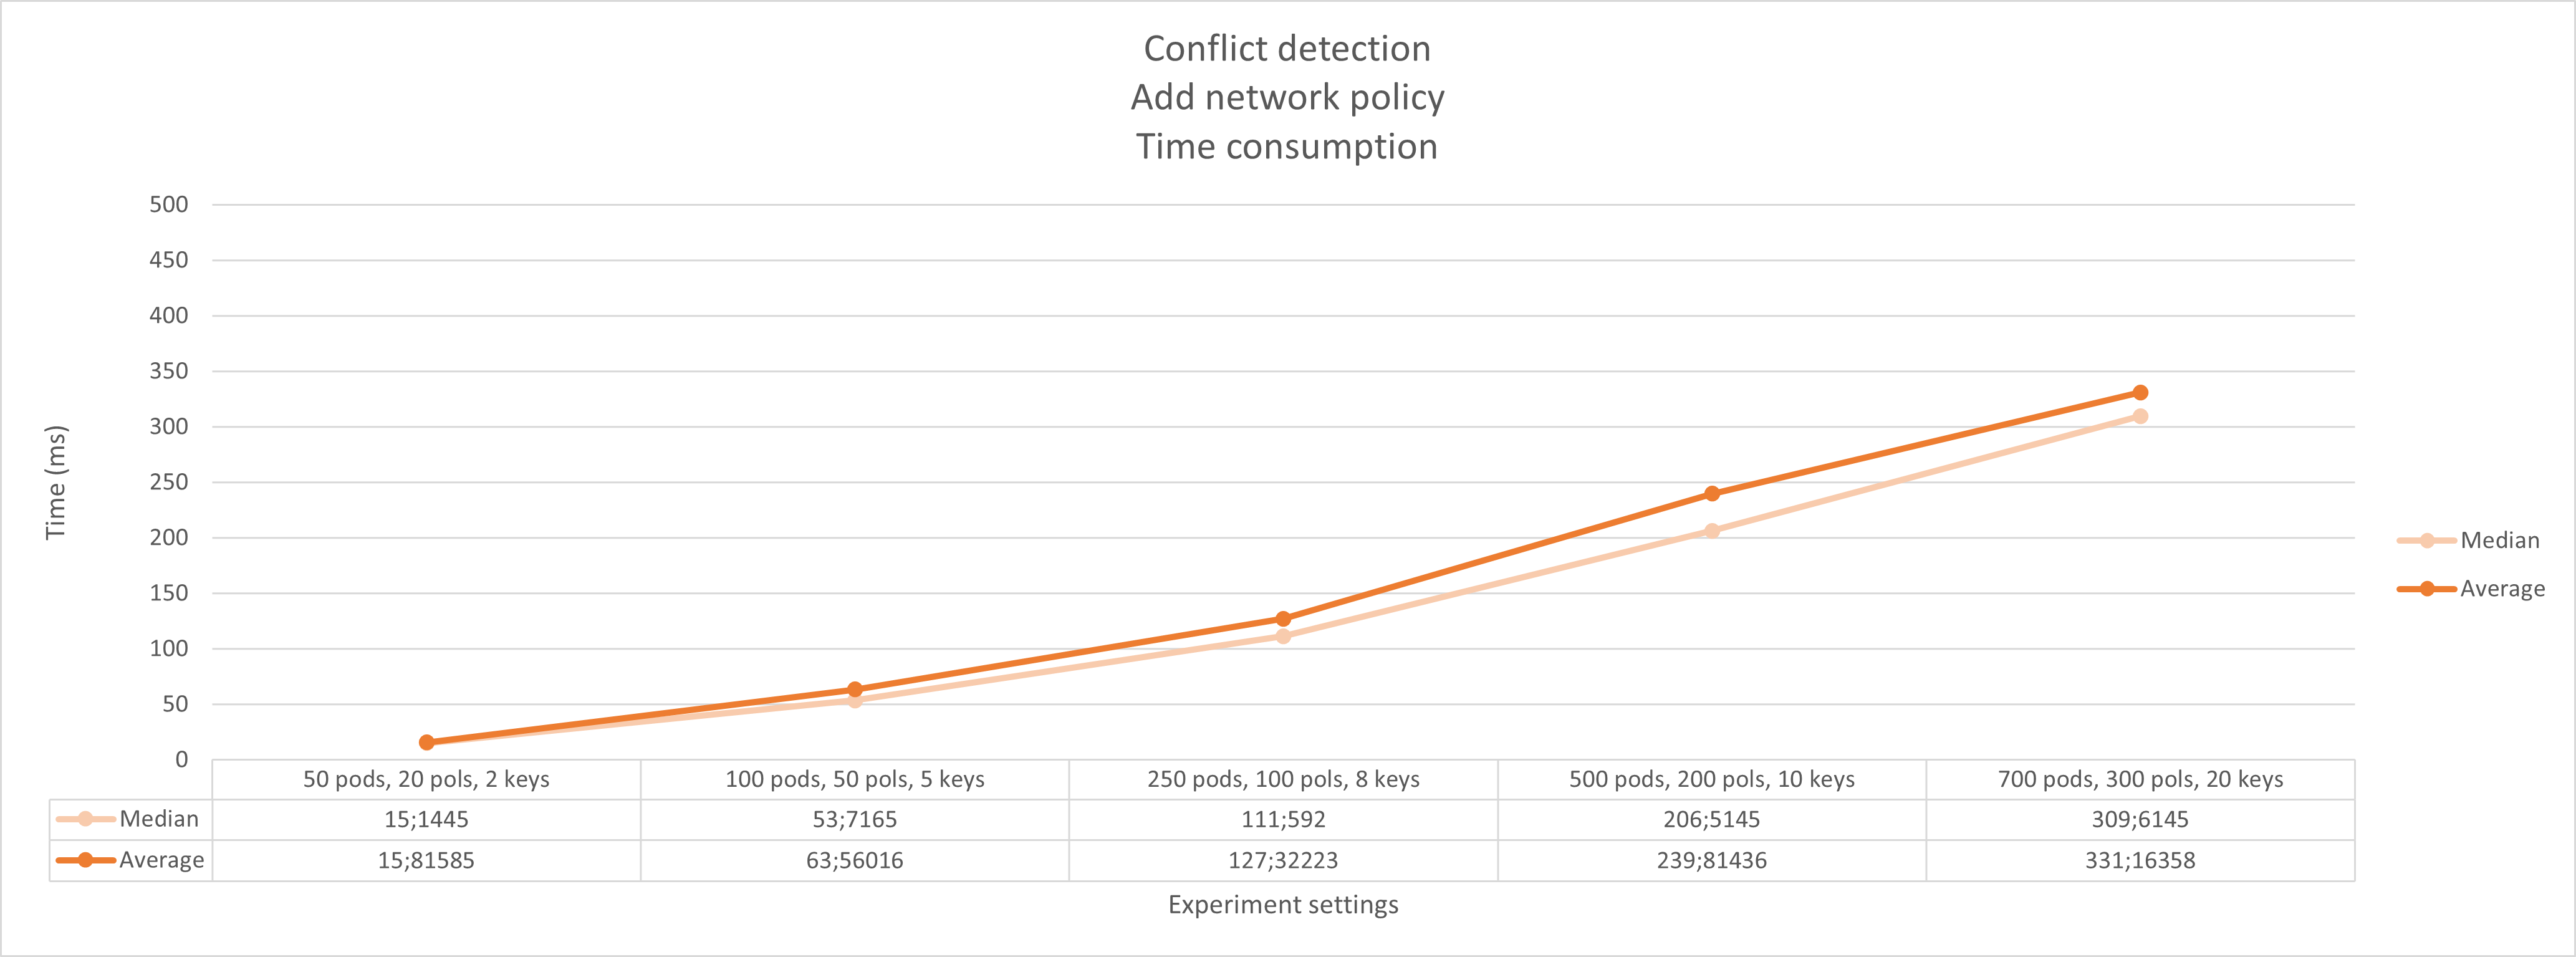
\includegraphics[width=\textwidth]{images/experiment2/addNP-time-conflict.png}
    \caption{conflict detection time consumption - add network policy}
    \label{fig:exp2-addNP-time-conflict}
\end{figure}
\begin{figure}[H]
    \centering
    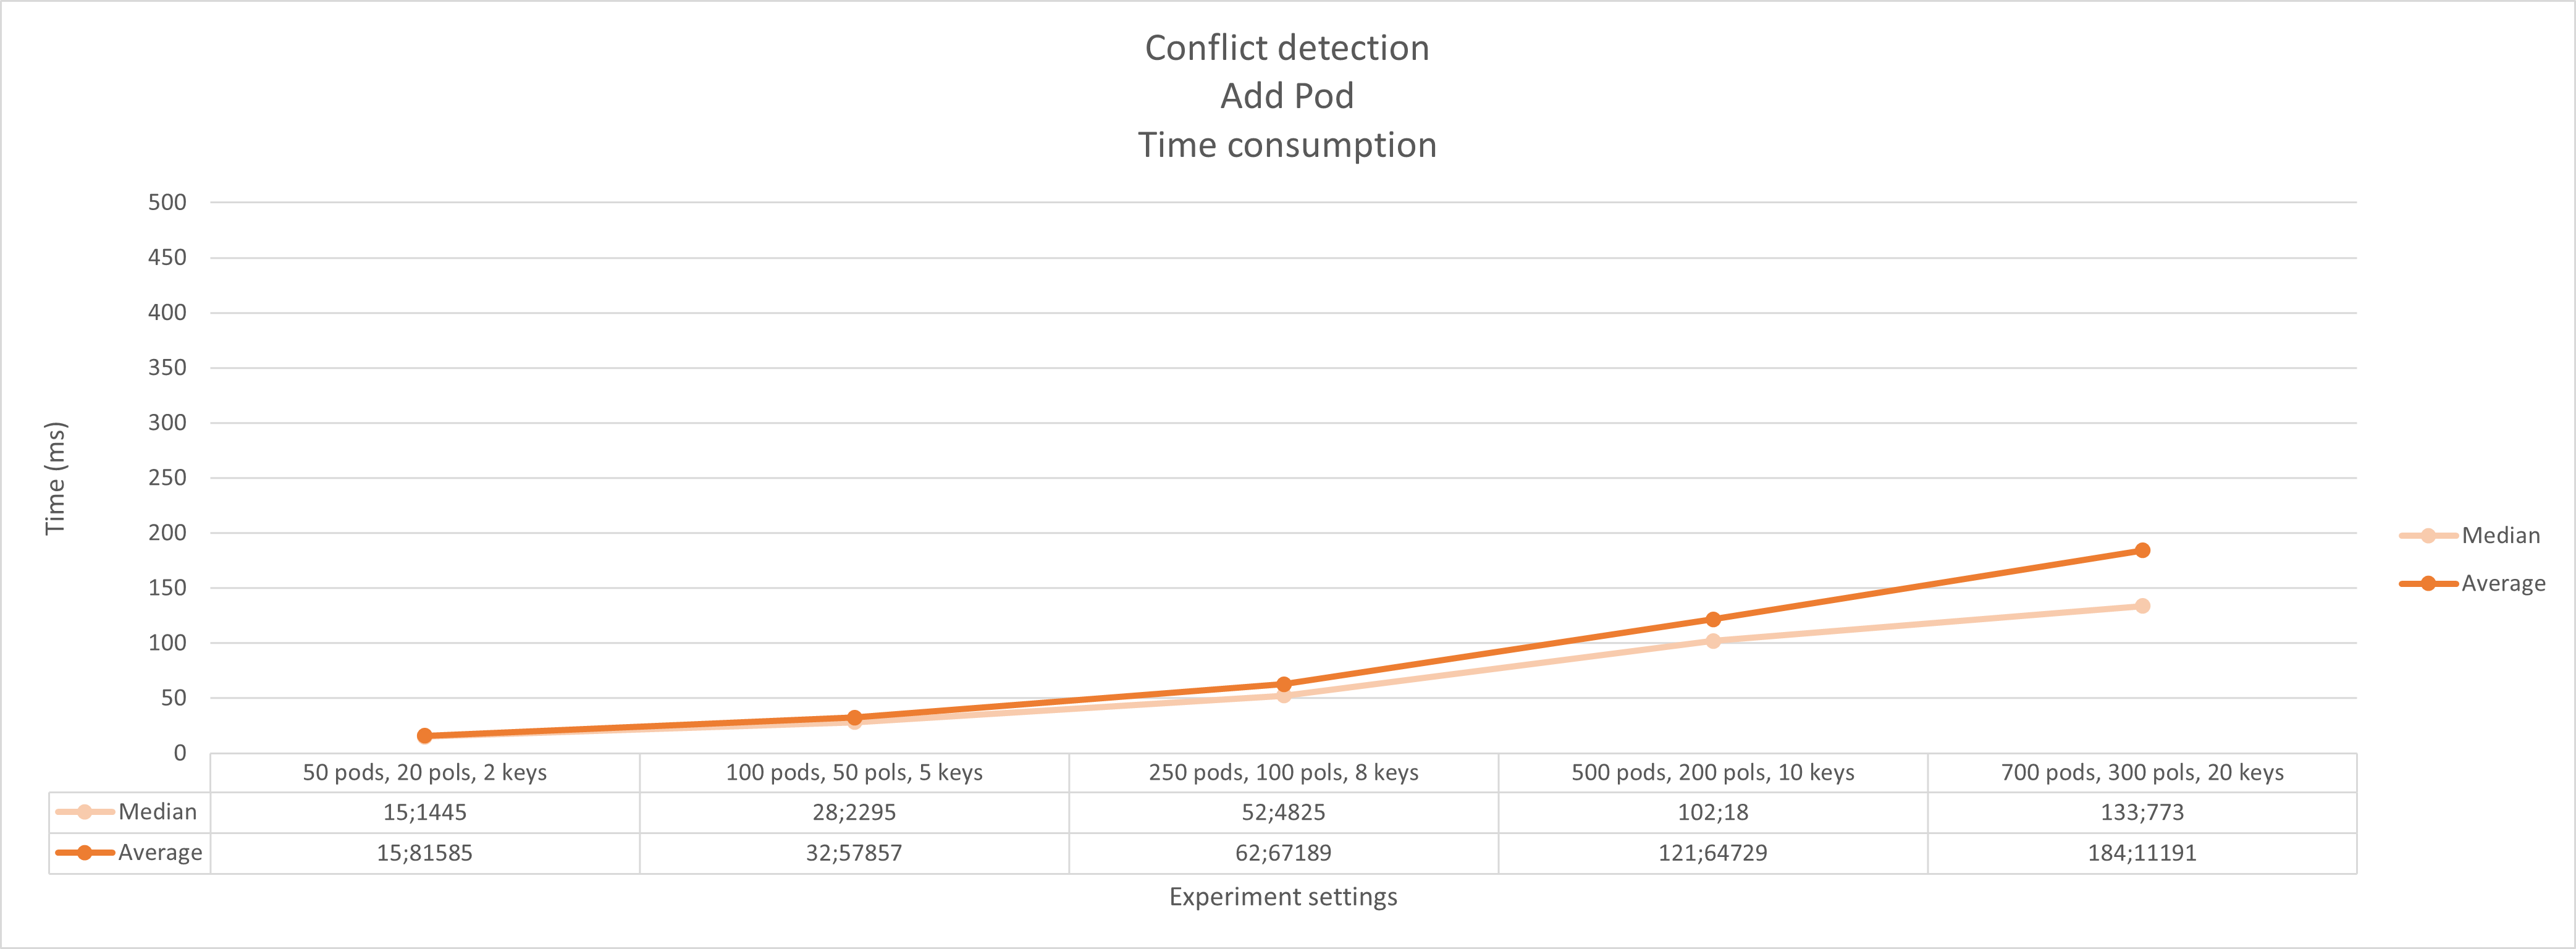
\includegraphics[width=\textwidth]{images/experiment2/addPod-time-conflict.png}
    \caption{conflict detection time consumption - add container}
    \label{fig:exp2-addPod-time-conflict}
\end{figure}
\begin{figure}[H]
    \centering
    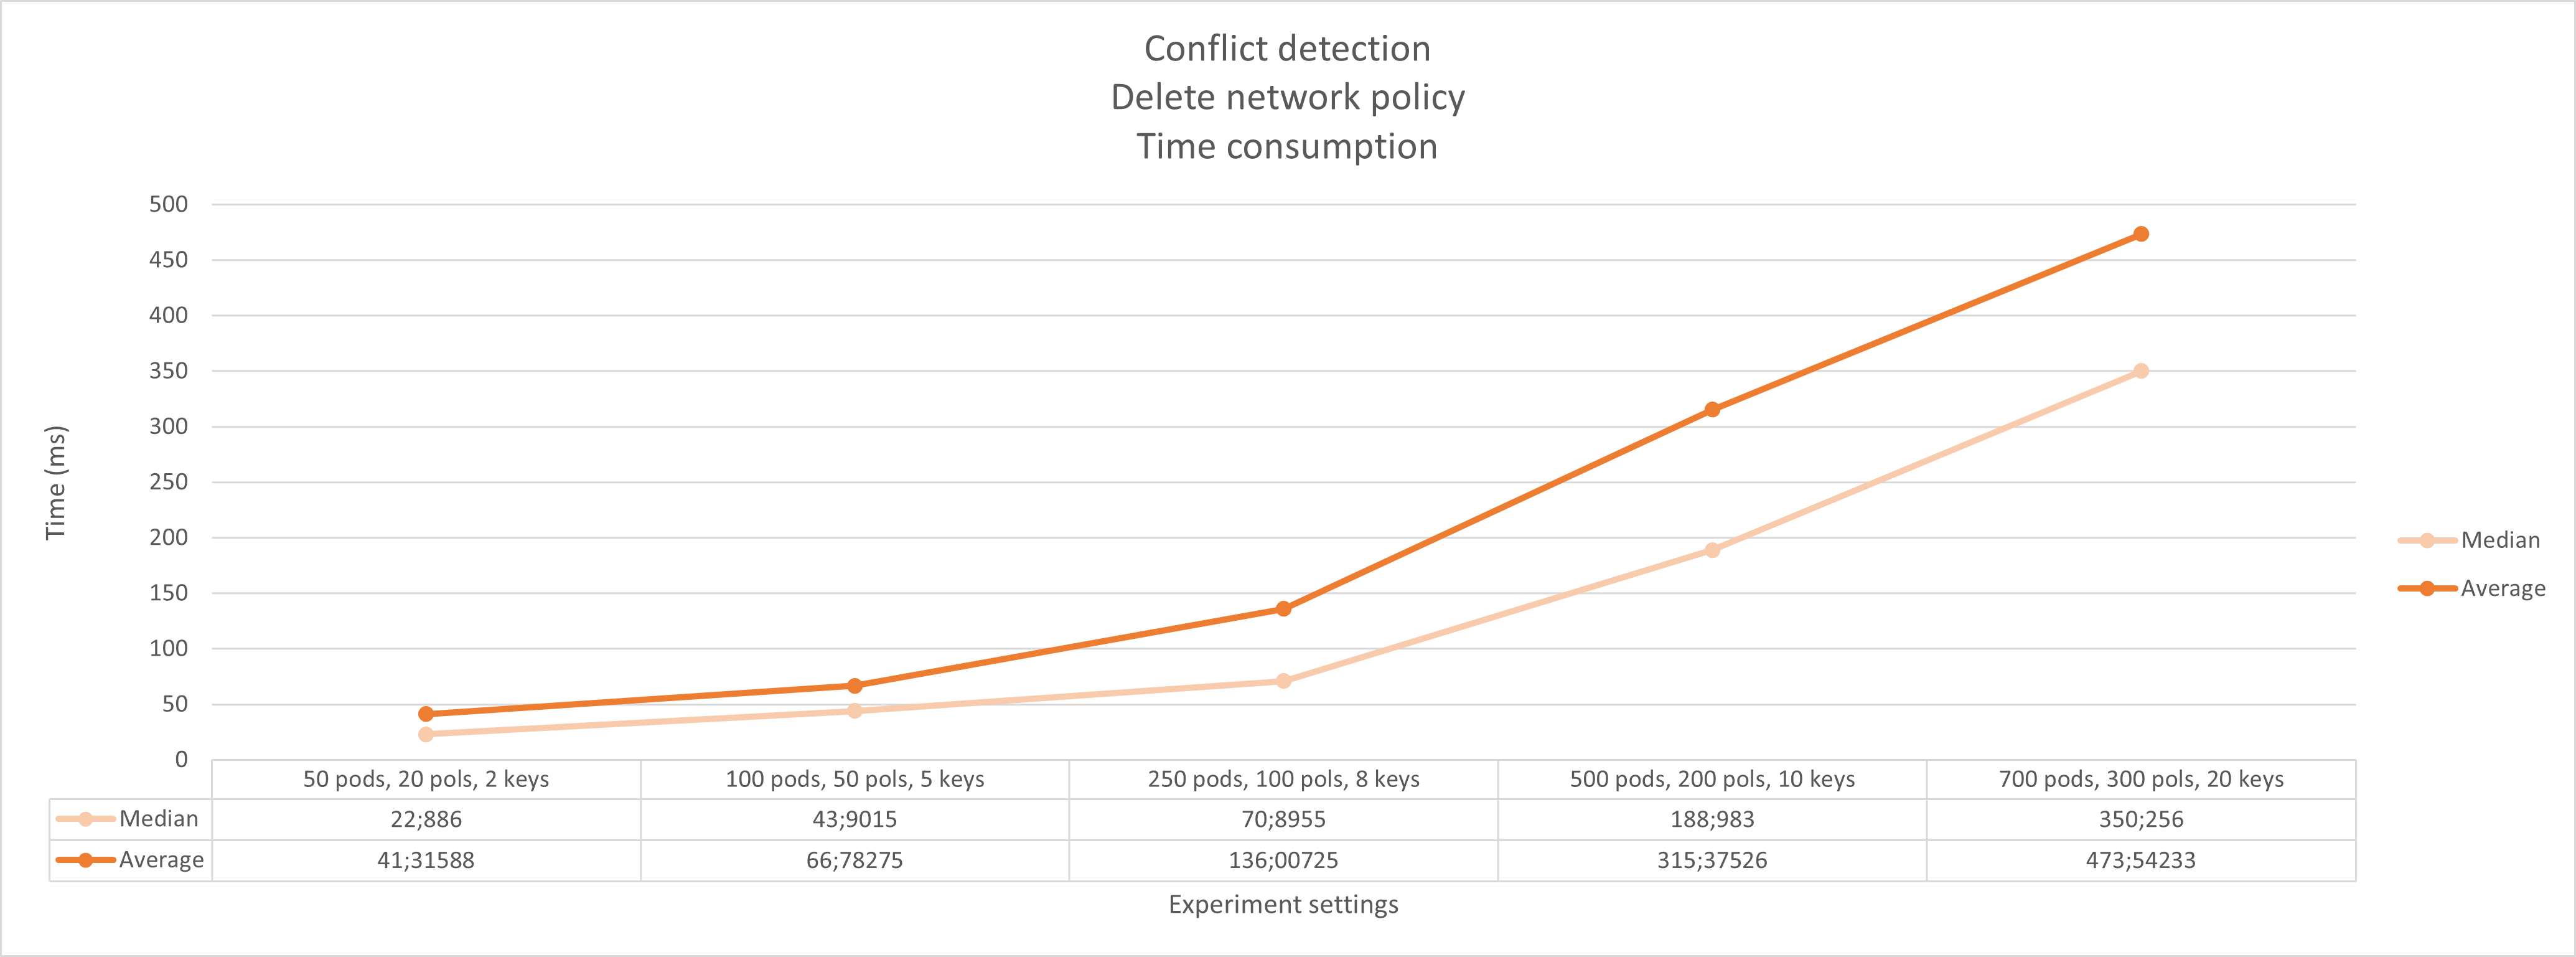
\includegraphics[width=\textwidth]{images/experiment2/delNP-time-conflict.png}
    \caption{conflict detection time consumption - delete network policy}
    \label{fig:exp2-delNP-time-conflict}
\end{figure}
\begin{figure}[H]
    \centering
    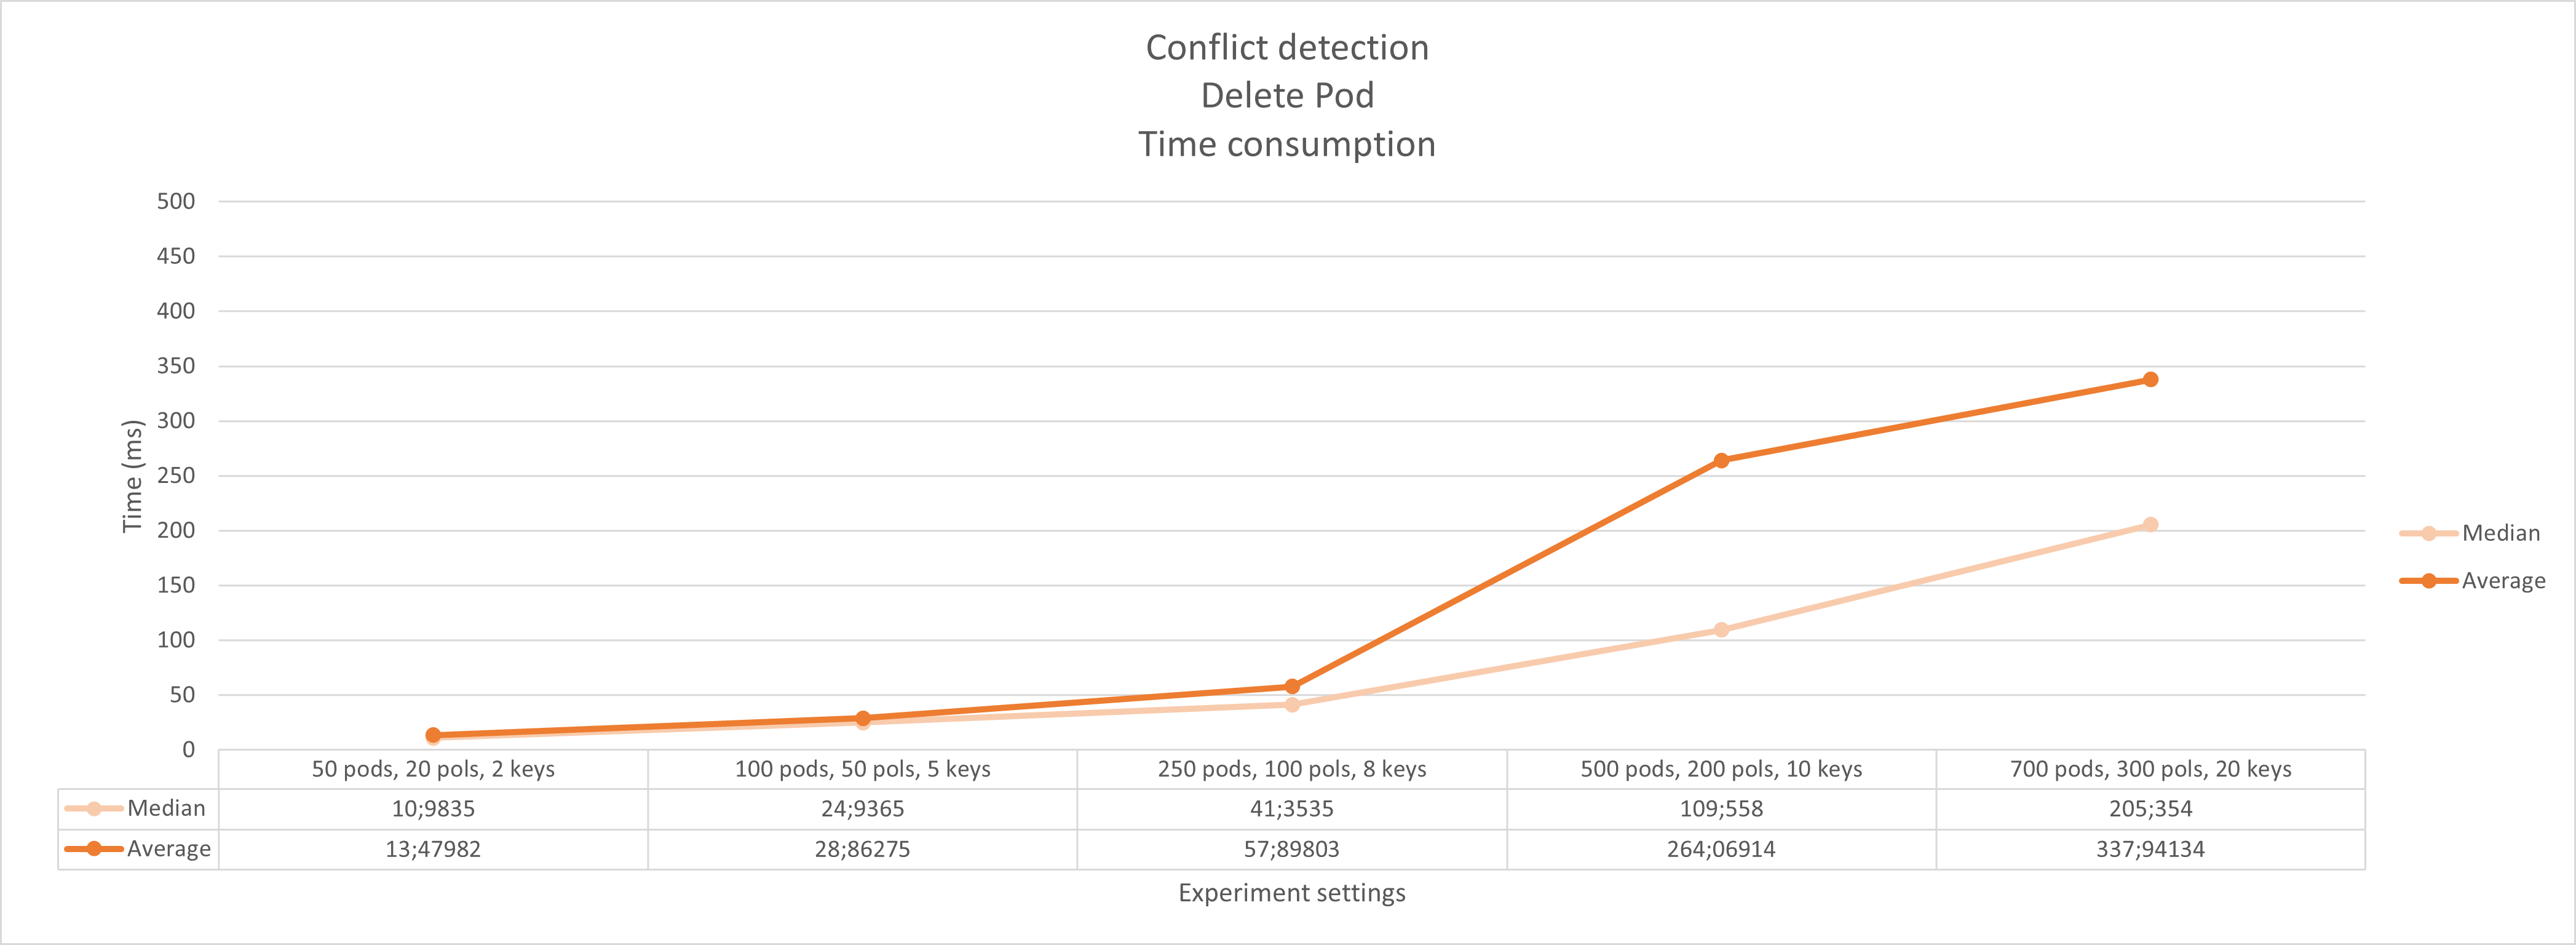
\includegraphics[width=\textwidth]{images/experiment2/delPod-time-conflict.png}
    \caption{conflict detection time consumption - delete container}
    \label{fig:exp2-delPod-time-conflict}
\end{figure}



\textbf{Memory consumption}
\newline The memory consumption for the full conflict detection solution for each of the four events are shown in \autoref{fig:exp2-addNP-memory-conflict}, \autoref{fig:exp2-addPod-memory-conflict}, \autoref{fig:exp2-delNP-memory-conflict} and \autoref{fig:exp2-delPod-memory-conflict}. The average values are usually in line with the median values meaning little to no skewing of data occurs due to outliers. One exception is the addition of a \acrshort{np} where the median lies higher than the average, which was also visible in the corresponding graph in experiment 1. We, therefore, assume that this is due to the incremental update of the cluster state and not because of the conflict detection itself, although an exact reason could not be found and would require extra experimentation. We conclude that some small differences between events can be found but there are no specific outliers that catch the attention and that the memory increases as the cluster grows in size which is in line with our expectation for Q4.

\begin{figure}[H]
    \centering
    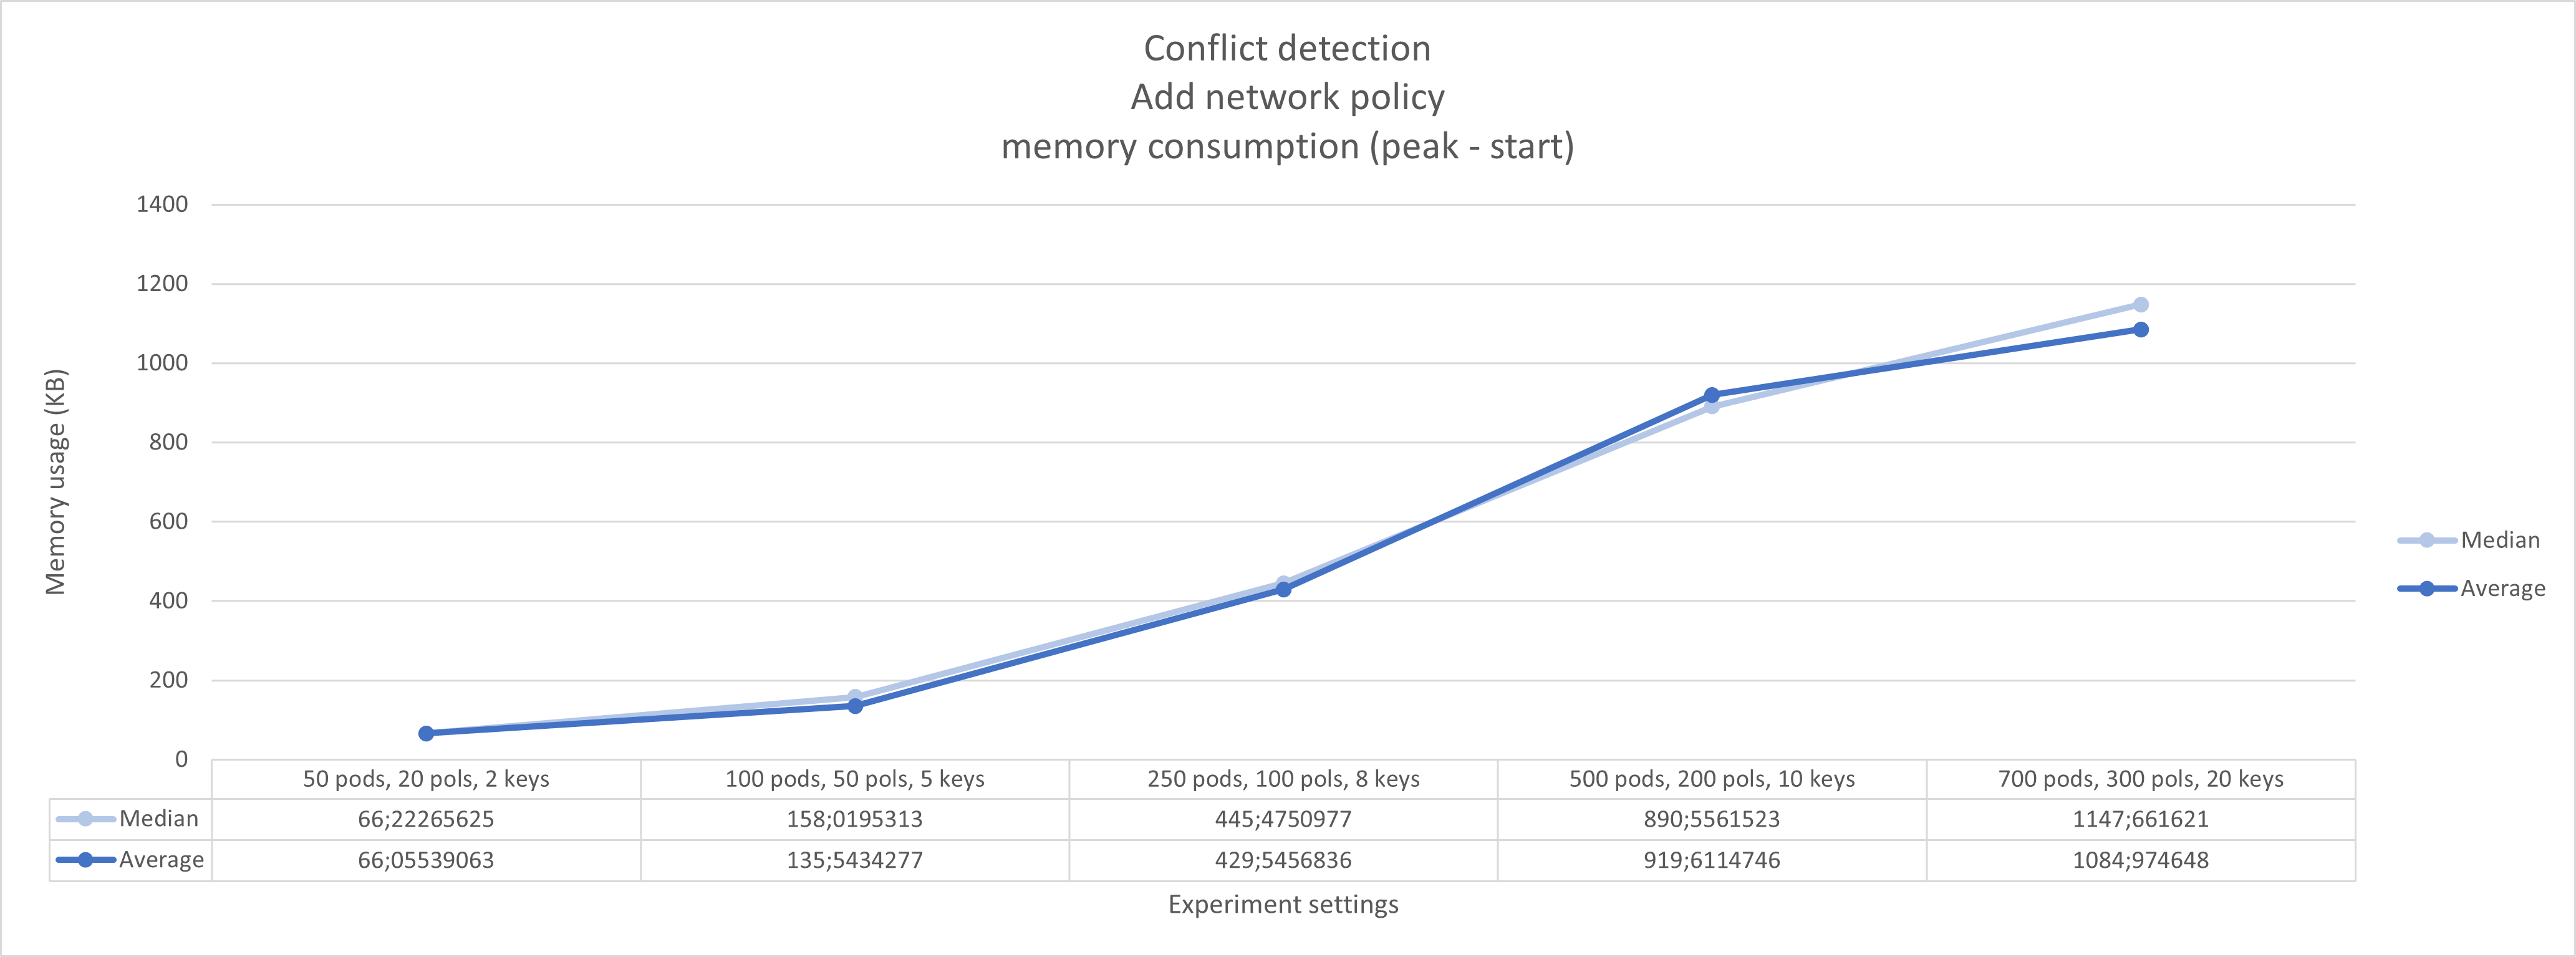
\includegraphics[width=\textwidth]{images/experiment2/addNP-memory-conflict.png}
    \caption{conflict detection memory consumption - add network policy}
    \label{fig:exp2-addNP-memory-conflict}
\end{figure}
\begin{figure}[H]
    \centering
    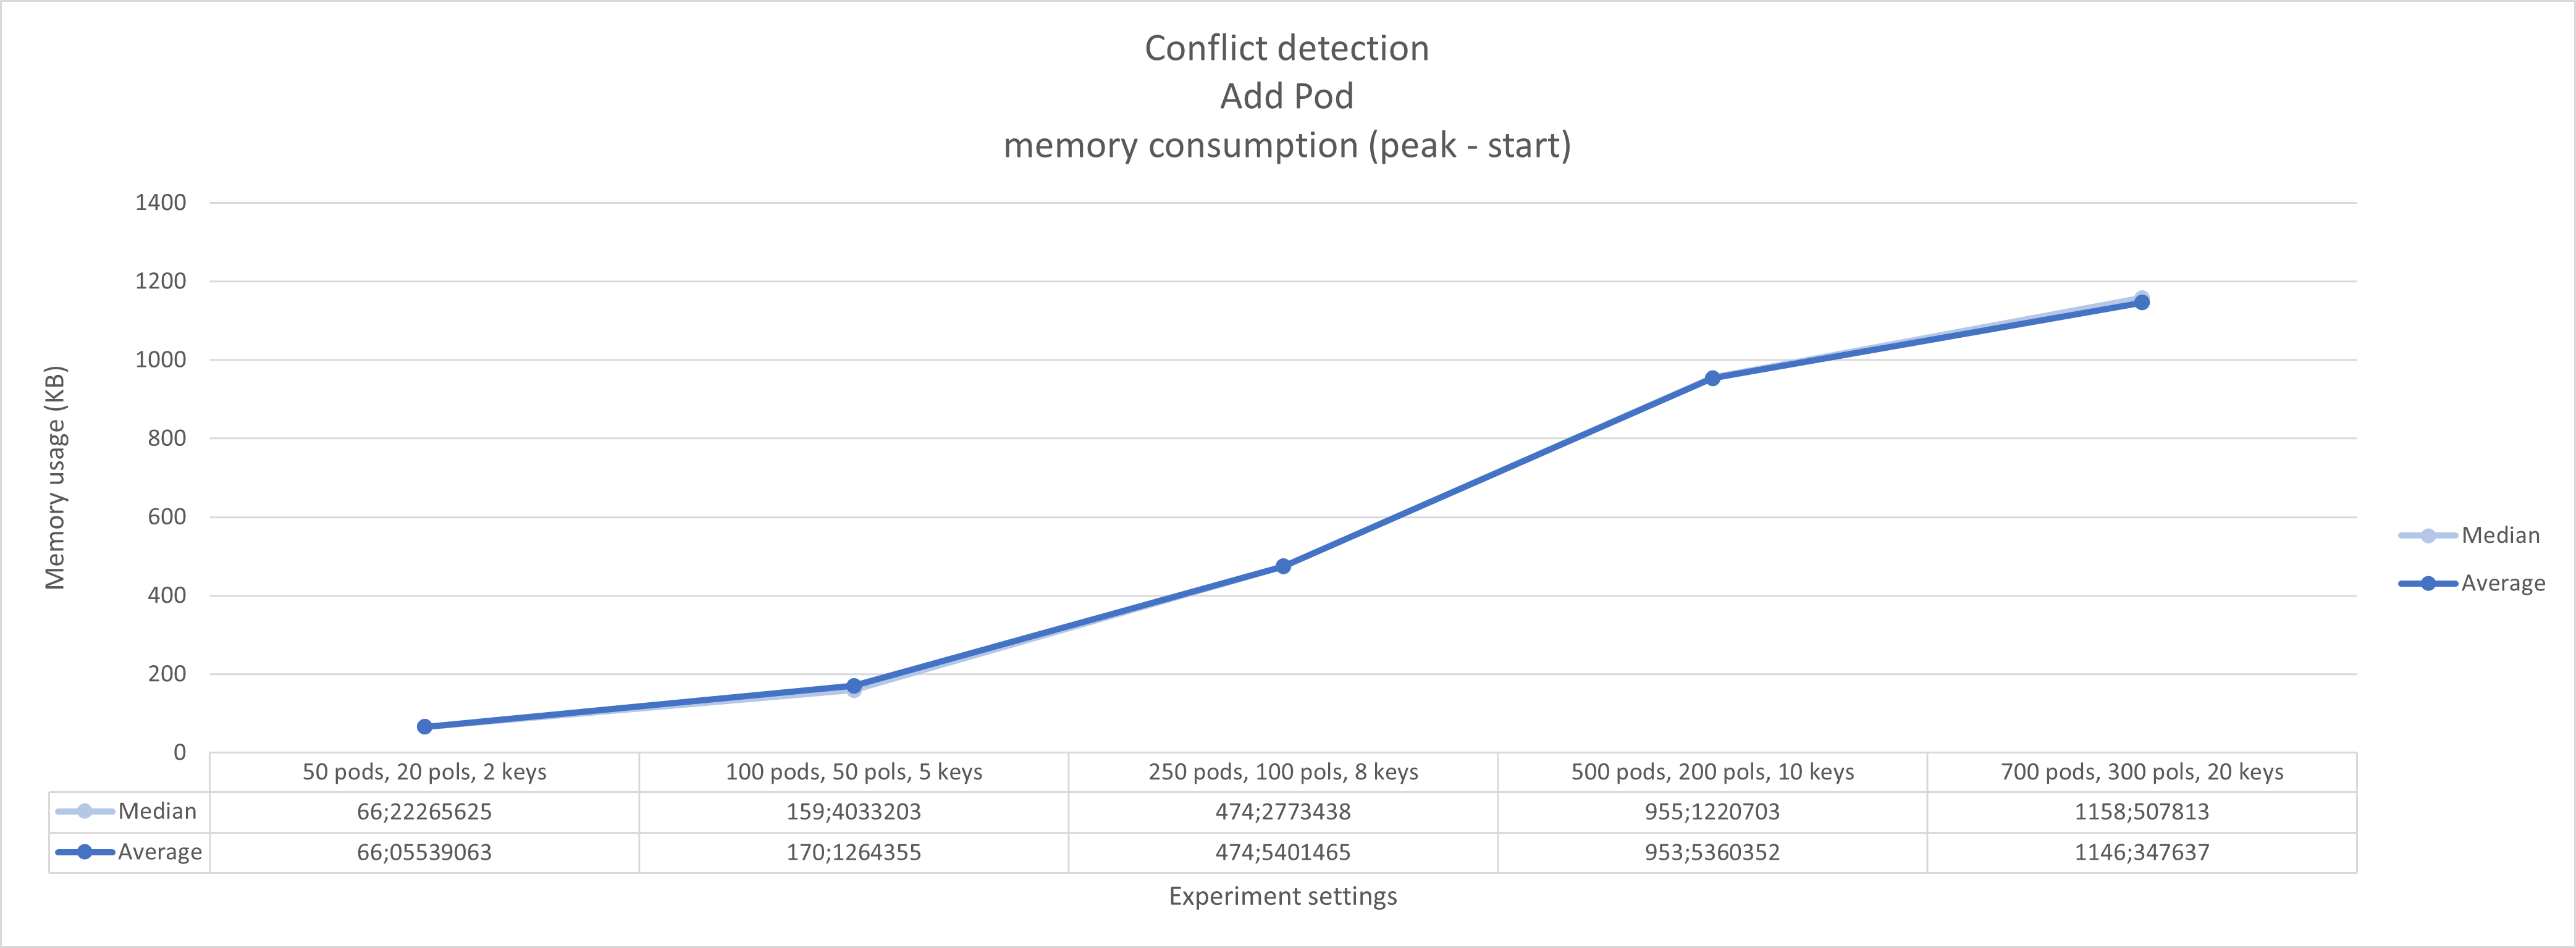
\includegraphics[width=\textwidth]{images/experiment2/addPod-memory-conflict.png}
    \caption{conflict detection memory consumption - add container}
    \label{fig:exp2-addPod-memory-conflict}
\end{figure}
\begin{figure}[H]
    \centering
    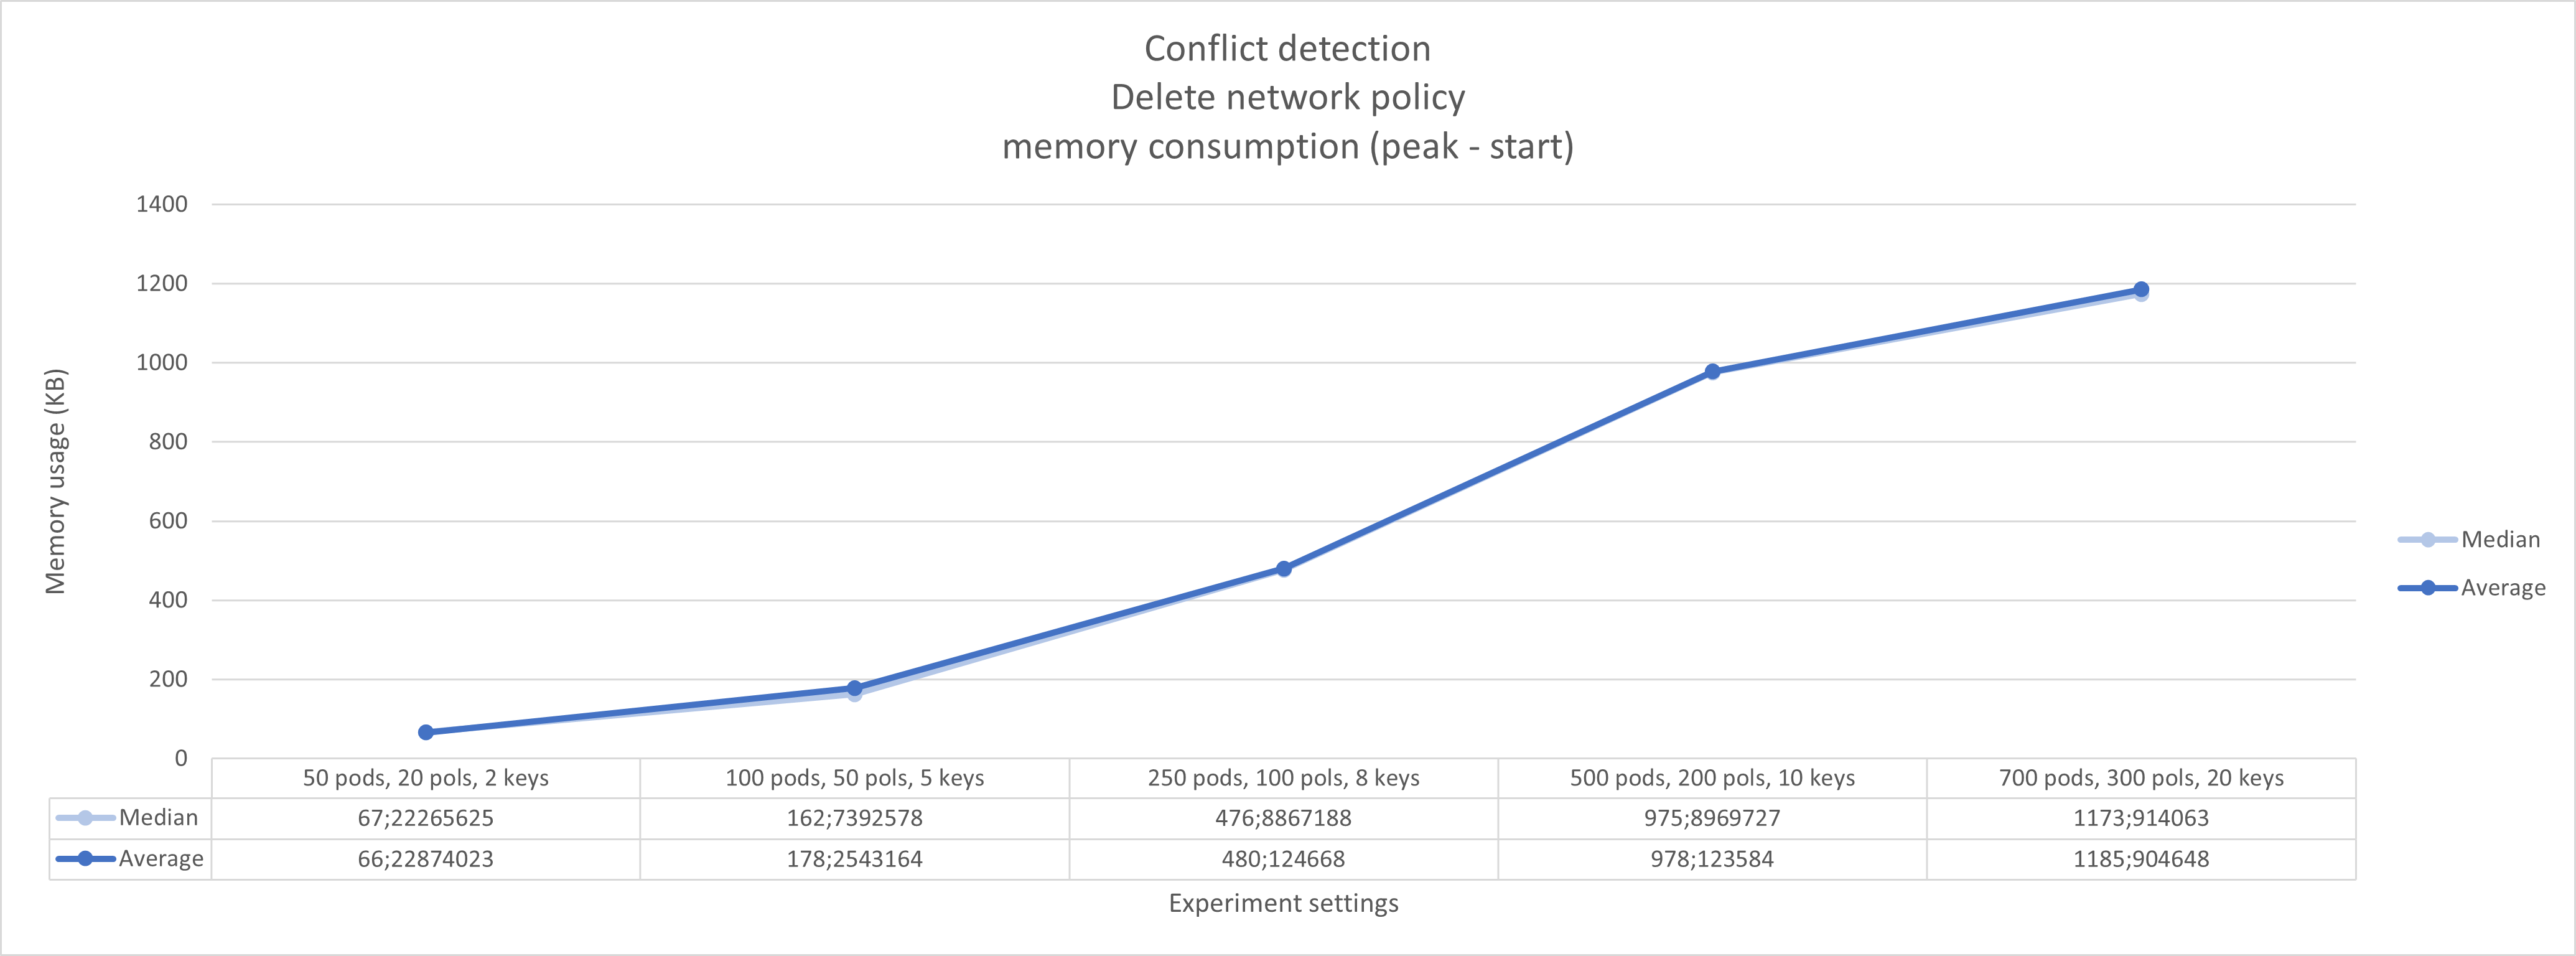
\includegraphics[width=\textwidth]{images/experiment2/delNP-memory-conflict.png}
    \caption{conflict detection memory consumption - delete network policy}
    \label{fig:exp2-delNP-memory-conflict}
\end{figure}
\begin{figure}[H]
    \centering
    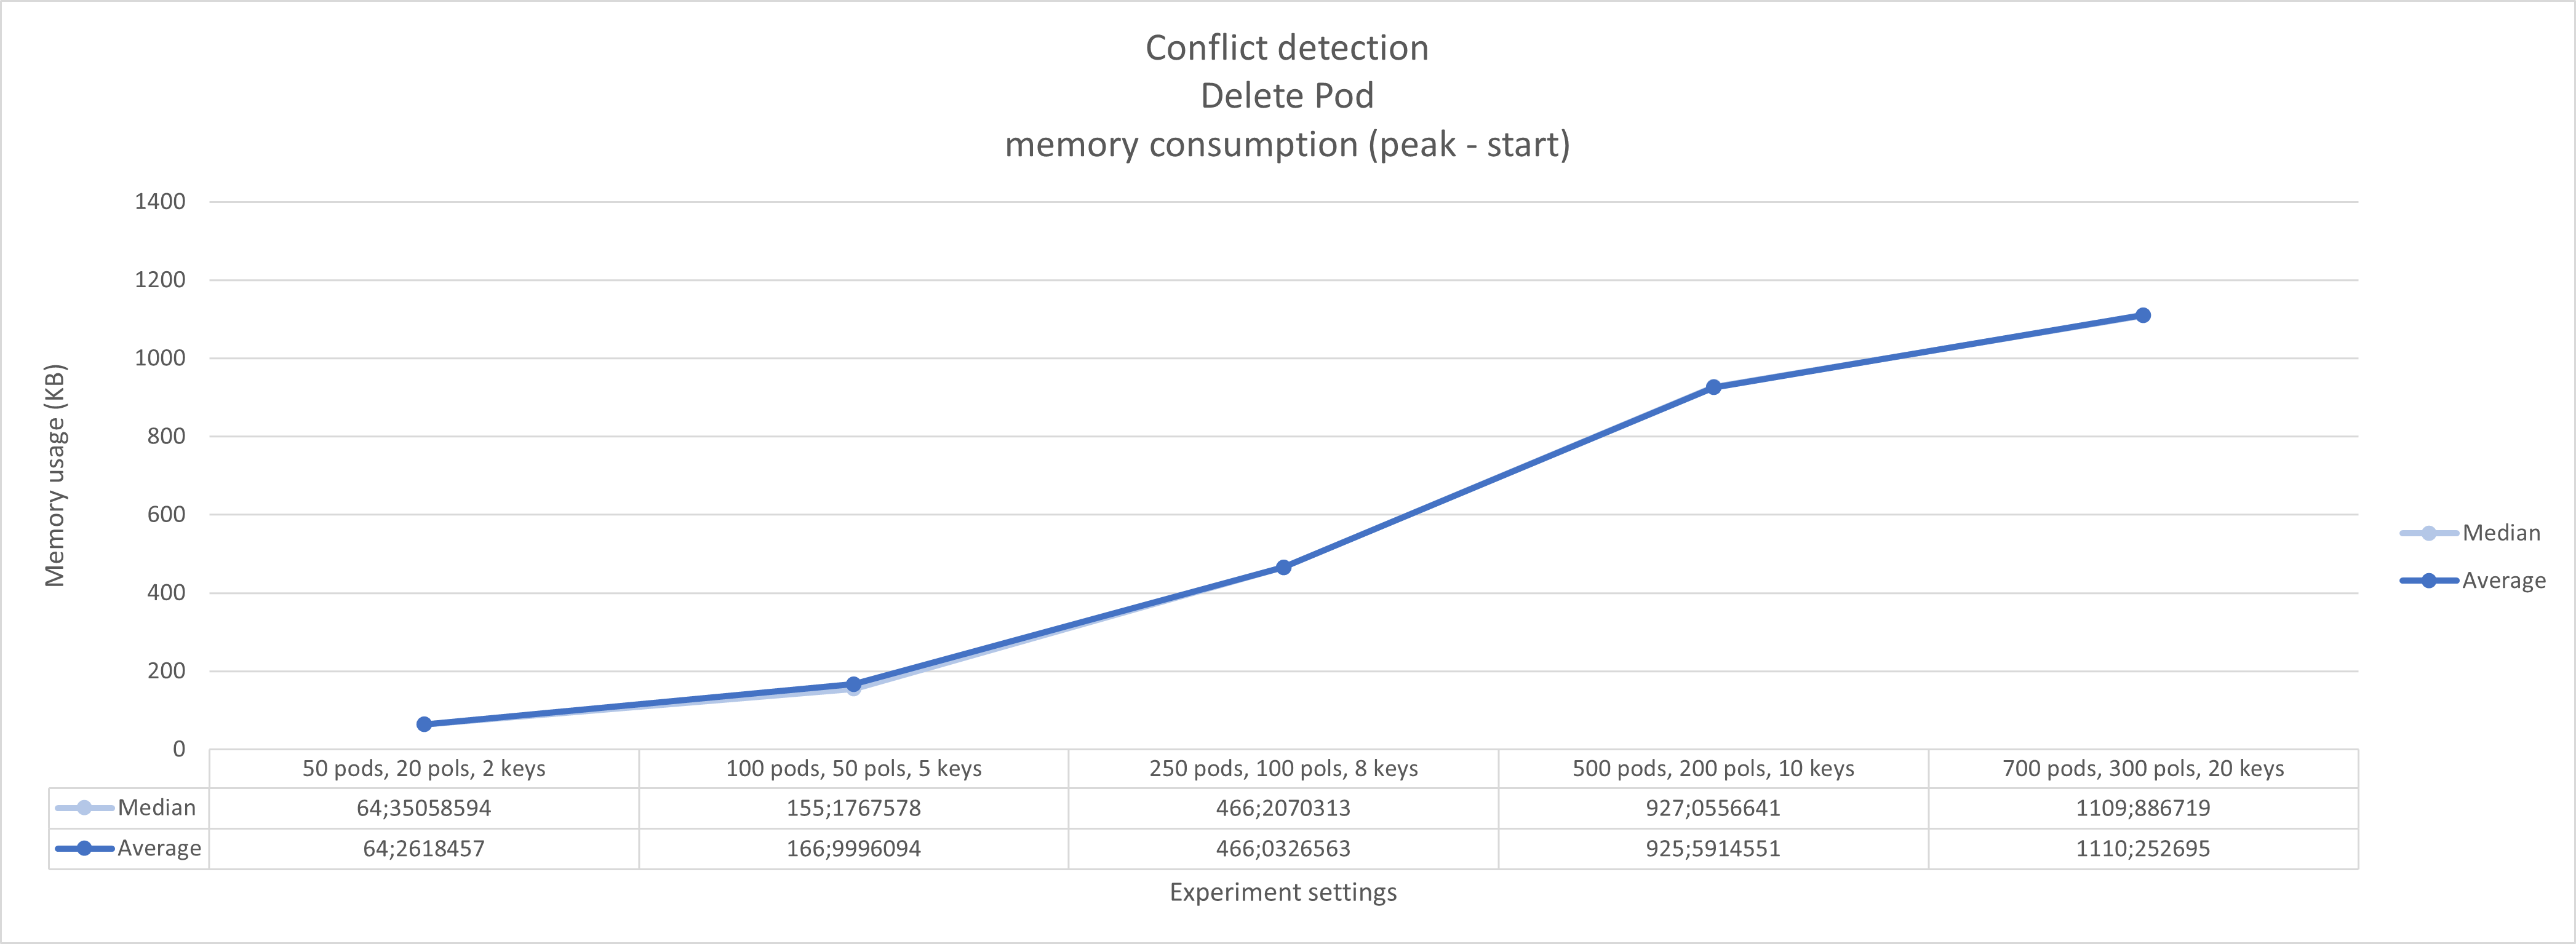
\includegraphics[width=\textwidth]{images/experiment2/delPod-memory-conflict.png}
    \caption{conflict detection memory consumption - delete container}
    \label{fig:exp2-delPod-memory-conflict}
\end{figure}


% =========================================
\section{Evaluation summary} \label{sec:conclusion}
We now combine the most important conclusions from these evaluation experiments into an overview:
\begin{itemize}
	\item Our incremental approach for updating the cluster state becomes faster than Kano's generative approach when we pass a certain cluster size threshold. This threshold changes depending on the cluster setup and the number of matches between label selectors in \acrshort{np}s and labels in pods. 
	\item The biggest drawback of the incremental update approach is the higher memory consumption due to the storage of the last cluster state compared to the generative approach. We must note however that the generative approach should be adapted to be usable for conflict detection in the algorithm and would require some extra variables which could lead to more memory usage as well.
	\item Updating the reachability matrix is the biggest contributor to time consumption whereas the conflict detection itself only adds slight overhead.
	\item Both memory and time consumption grow as the number of containers and \acrshort{np}s in the cluster increases. The biggest contributor to time consumption is the number of connections between containers that are defined by network policies.
\end{itemize}

\cleardoublepage
